\documentclass[acmlarge]{acmart}
% alternate title: ML for Phone-Based Relationship Estimation: Considering Location Semantics and Population Heterogeneity
\title{Machine Learning for Phone-Based Relationship Estimation: The Need to Consider Population Heterogeneity}
\date{}
\author{}

% TODO have to make sure that the packages play nice with the latex template format
% \usepackage{amsmath}
% \usepackage{float}
% \usepackage[margin=1in]{geometry}
% \usepackage{graphicx}
\usepackage{hyperref}
% \usepackage[utf8]{inputenc}
% \usepackage{multicol}
%\usepackage{natbib}
%\usepackage{titlesec}
% \usepackage{xcolor}

%\titlespacing*{\section}{0pt}{0.5\baselineskip}{0.5\baselineskip}
%\titlespacing*{\subsection}{0pt}{0.5\baselineskip}{0.5\baselineskip}

\begin{abstract}
%IMWUT abstract length: 150-200 words
Estimating the category and quality of interpersonal relationships from ubiquitous phone sensor data matters for studying mental well-being and social support. Prior work focused on the volume of communications to estimate broad relationship categories. Here we contextualize communications by combining phone logs with demographic and location data to predict interpersonal relationship roles, producing better performance ($F1=0.68$) than using communication features alone. We also explore the effect of age variation in the underlying training sample on interpersonal relationship prediction and find that models trained on younger subgroups, which is popular in the field, generalize poorly to the wider population. Our results not only illustrate the value of using data across demographics, communication patterns and semantic locations, but also underscore the importance of considering population heterogeneity in phone-based personal sensing studies.
\end{abstract}

\begin{document}

\maketitle

\section{Introduction}
\label{sec:intro}
% Why care about estimating relationships?
Being able to understand the nature of interpersonal relationships and phone-based communication can be useful for studies of mental health. Studies have shown connections between perceived social support within relationships and effects of stress~\cite{cutrona1987provisions}, mood disorders such as depression~\cite{george1989social}, and psychological disorders such as schizophrenia and substance abuse~\cite{salyers2001social}. An individual's interpersonal context can be an indicator or risk factor: depressed individuals exhibit asymmetric communication patterns where they are less likely to initiate social interactions~\cite{hames2013interpersonal} while individuals with a strong support network are less prone to depressive episodes. The social role a specific contact plays is critical, as a call from work provides a vastly different kind of interaction and social support to an individual than a call from a friend. 

% Role/Advantages of passive-sensing
With the proliferation of smart mobile devices that passively collect data on user behavior~\cite{harari2017smartphone}, there is an increasing interest in estimating behavioral markers like social communication context through passive sensing~\cite{lane2010survey,mohr2017personal}. Automated analysis of such passive data can potentially provide avenues for early detection of mental health~\cite{canzian2015trajectories}. If an automated process could detect elevated risk factors for mental health in a person, that individual could be targeted for a more thorough assessment (and provided with digitized forms of support and treatment), alleviating many of the constraints associated with traditional assessment methods~\cite{suchman1962analysis}.

% Prior work and gaps
Previous works in passive sensing to estimate social relationships, tie strength, and friendship networks have used feature modalities such as communication logs, Bluetooth proximity, and geo-location tags to build machine learning models~\cite{eagle2009inferring,min2013mining,wiese2015you,hsieh2014inferring}. However, many of these studies focus on broad social categories (such as friend vs. not friend~\cite{eagle2009inferring}, and social vs family vs work~\cite{min2013mining}) where there could be overlap between roles or contacts that do not fit cleanly into a category. Moreover, we currently know little about the relationship of communication events with demographic and semantic location information, which could reveal additional fine-grained relationship information. We need to learn more about fine grained aspects of relationship and its generalization across demographics.

Furthermore, machine learning is not a cure-all, especially given the small sample sizes in the mobile personal sensing literature. Previous meta-analyses revealed that most papers utilize spurious baselines that lead to false optimism in the model results~\cite{demasi2017meaningless}. As machine learning tools become more ubiquitous and accessible, there is also a concern that methods are incorrectly applied. A literature review focusing on phone sensing models found that improper record-wise cross-validation which overestimates performance is frequently utilized in this space~\cite{saeb2016voodoo}. More generally, there is the issue of replication: studies are often conducted on a narrow group such as college students~\cite{eagle2006reality, wang2014studentlife} that may not generalize to a wider population~\cite{mohr2017personal}. Our goal is not just to produce good machine learning results but also to build generalizable models that are clinically and statistically meaningful.

% Our contributions
To address these gaps, we take a principled approach to social role prediction by contextualizing communication events with location and demographic data on a larger participant population ($n=199$) collected from across the United States. We make the following contributions:

\begin{itemize}
    \item We use \textit{auto-sklearn}, an automated machine learning technique~\cite{feurer2015efficient}, to build our models in order to reduce the biases introduced by manual model and feature selection.
    \item We contextualize participant's communication patterns with semantic location information and demographics, achieving a weighted F1 score of 0.68 on a held-out test set.
    % TODO more emphasis on age interactions
    \item We perform feature analysis and show that there are significant correlations between both the temporal tendency and channel selection of communication patterns and the age of the participants.
    \item We present an experiment where models are trained only on subsets of the population divided into age quartiles to illustrate the impact of population heterogeneity on model performance.
\end{itemize}

The rest of the paper is organized as follows. We review related work in Section~\ref{sec:related_work} and describe our data collection, feature extraction, and modeling methodology in Section~\ref{sec:methods}. In Section~\ref{sec:rel_pred_results}, we present our relationship prediction modeling results and analyze feature importance as well as correlations in communication patterns. We introduce our subgroup prediction task and subsequent performance analysis in Section~\ref{sec:subgroup_results}. We conclude by discussing implications of our results as well as limitations in Section~\ref{sec:discussion}.

% TODO ideally have an auto-sklearn citation for overengineering

\section{Related Work}
\label{sec:related_work}

% \textbf{Thread of gaps throughout related work}
% \begin{itemize}
%     \item small n studies with students for relationship prediction
%     \item focus on communication features and colocation information (symmetric relationships, not easily obtained), relatively little focus on semantic location which can be more easily obtained
% \end{itemize}

The ubiquity of personal sensing platforms has provided an opportunity for many novel modeling methods of human social behavior. In particular, there have been numerous previous studies for predicting relationship roles or social network analysis through passively collected phone data spanning different sensor modalities, such as bluetooth and communication logs. However, many of these studies also use data drawn from student or university participants, which are not representative samples of the wider population. We review prior work here to examine the breadth of model features as well as sample populations used in the literature.

% sample analysis of prior work: predominantly student populations 
Understanding the composition of the underlying sample population is important for the evaluation of a predictive model's generalizability. An influential work in estimating social systems using phone sensors, Reality Mining~\cite{eagle2006reality}, gathered bluetooth proximity, usage, and communication data from an academic population, where the 94 participants in the study were affiliated with MIT. Groups have used this public dataset to predict friend vs non-friend relationships with high accuracy through a variety of features such as spatial proximity~\cite{eagle2009inferring} and communication logs~\cite{mirisaee2010mining} as well as through novel modeling settings such as semi-supervised network inference~\cite{yu2017semi}. Numerous other works have leveraged student samples to produce effective relationship prediction models, albeit at small sample sizes~\cite{reinhardt2015show,hsieh2014inferring,dwarakanath2016analyzing}, and other similar works with different inference targets such as social support~\cite{ghosh2018modeling}, depression assessment~\cite{lu2018joint}, and happiness~\cite{jaques2015predicting} have also been extensively explored within students as well. Though academic populations are accessible for research groups, models trained on these data may not produce results that can ultimately generalize to other samples of differing demographics or even of different academic institutions.

% TODO weak CCC context
% more heterogenous samples -> still not enough
There are other studies that have collected samples from more heterogeneous populations: Min et al~\cite{min2013mining}'s study of predicting \textit{life facets} (family, work, social) from phone data as well as a follow-up study of tie strength~\cite{wiese2015you} use a sample of 40 participants recruited across the United States, though they are still majority students. Choi et al~\cite{choi2013mining} mine relationship types from 22 participants within a workplace environment, though their population is homogeneous in other aspects: 20 of the participants were male and all were computer science majors. The data used by the CommSense phone mining framework~\cite{bao2015commsense} crowd-source their sample of 106 users from geographically diverse areas in the United States. Overall however, a vast number of studies in the personal sensing space draw from small, homogeneous samples that are skewed towards a particular demographic.

% standard communication features and colocation data
% TODO not sure if highlighting shortcomings of co-location information buys us anything in the argument
% TODO CCC context
Across previous relationship prediction work, the primary modeling features utilized are communication patterns extracted from text message, call, email, and instant message logs which are easily accessed through phone sensor data platforms~\cite{mirisaee2010mining,dwarakanath2016analyzing}. Co-location information is also often used to infer social network structure~\cite{eagle2009inferring,yu2017semi,hsieh2014inferring,choi2013mining}. However, co-location information requires ``symmetric'' data (from both target participants and their contacts) to be collected which would be more difficult to collect at scale or when participants are not spatially located in a similar geographic area. Part of the appeal of personal sensing is that data like communication logs are much easier to collect, making subsequent prediction models applicable to a wider range of source data and populations.

% additional demographic, and location features
Though phone communication patterns can be indicators for the nature social relationships, differences in how users behave (eg due to life stage) or missing context (eg communications while traveling) potentially limit the predictive of communication features alone~\cite{wiese2015you}. Previous studies address this by leveraging other sensor modalities in addition to communication features to improve their models. Min et al include demographic information (age, gender differences) as well as survey results that capture additional relationship information such as closeness, finding that the combination of this information with communication fetures produced the best predictive performance~\cite{min2013mining}. The CommSense system uses basic semantic location information to contextualize communication events, with labels for calls or texts that occur at home or at work~\cite{bao2015commsense}. Overall however, inferring social relationships with other features such as demographics and location needs to be explored further, as these data are easily collected through personal sensing platforms and can better characterize communication patterns.

% how our study is unique: larger sample, heterogeneous population, semantic location information
% TODO feels a bit like a recapitulation of the contributions in the intro
% TODO CCC conclusion
Our work builds upon these existing studies by introducing fine-grained demographic and user-categorized location features for relationship prediction on a large, heterogeneous dataset. Though our location labels are more detailed than the high-level work vs home vs other categories used in CommSense, previous work by Saeb et al has demonstrated that semantic location can inferred from phone sensor data with good performance~\cite{saeb2017mobile}, making these features viable for use in other personal sensing studies.

Our work also makes contributions from a modeling perspective by using automated machine learning methods~\cite{feurer2015efficient} --- Lane et al note that most groups in the personal sensing space use hand-coded and hand-tuned models, which lead to questions on not how well these models generalize but also on how these models can be shared and standardized~\cite{lane2010survey}. Automated machine learning methods are powerful but also limit the user intervention when training and building predictive models, which could provide a common platform for the evaluation of various personal sensing tasks going forward.

Additionally, we note that the vast majority of these studies use small $n$ samples that are primarily drawn from student populations, which are often homogeneous demographically, particularly in terms of their age distribution. Our age-based subgroup experiment presented in Section~\ref{sec:subgroup_results} will explore the impact of training on such homogeneous samples, highlighting the need to collect data from more varied populations in order for personal sensing models to generalize.

\section{Methods and Data}
\label{sec:methods}
%The question we wish to answer is: can we predict contact communication roles and tie strength using passively collected phone features? We consider semantic location, demographics, and communication feature modalities as well as various target predictions: higher level three-class social role classification, finer-grained six-class social role classification, as well as classification and regression of contact tie strength. We leverage \textit{auto-sklearn} throughout all our experiment settings.

\subsection{Data Collection}
\label{subsec:data_collection}

% TODO elaborate on data collection methodology
Our dataset consists of 199 individuals (163 female, 33 male, 3 other) recruited between October 28, 2015 and February 12, 2016 across the United States that were at least 18 years old ($\mu = 38.27 \text{ yrs}, \sigma=10.19$), owned an Android smartphone (OS 4.4 through 5.1), and had access to WiFi. Individuals with psychotic disorders, inability to walk half a mile, or positive screens for alcohol abuse were excluded from our study. Participants were enrolled in the study for six weeks, where they installed \textit{Purple Robot}~\cite{purplerobot}, an open source Android application for recording phone sensor data, on their devices. 

% TODO flesh out with codebook information
\subsubsection*{Passive sensing}
Call and text information was logged, including whether the communication was incoming, outgoing, or missed as well as the total call duration. 

\subsubsection*{EMA and survey data}
In addition to the passive data collection, participants responded to EMA surveys that asked questions about semantic location as well as the contacts they communicate with. After the conclusion of the first logged communication, contacts were labelled with one of seven possible options:

\begin{itemize}
    \itemsep0em 
    \item Significant Other
    \item Friend
    \item Family Member You Live With
    \item Family Member You Don't Live With 
    \item Colleague/Work-Related
    \item Task (e.g. Make an Appointment, Reservation, etc.)
    \item Other
\end{itemize}

% Given that we're not focusing on tie strength for this paper, this should be omitted?
% Additionally, participants answered short questionnaires for each contact on a seven point Likert scale:

% \begin{itemize}
%     \itemsep0em 
%     \item How much did you want to communicate with this person today?
%     \item I would talk to this person about important matters
%     \item I would be willing to ask this person for a loan of \$100 or more.
%     \item How close are you to this contact?
% \end{itemize}

In total, for our participants we have 9,645 recorded contacts across 52,850 calls and 353,467 SMS messages. 
% TODO summarize basic distributions with a histogram, or ranked order plot
The number of contacts per participant is varied, with ranges from a single contact to 159 contacts (25th percentile: 24, 50th percentile: 37, 75th percentile: 58).

\subsection{Prediction Target: Top Five Contacts}
\label{subsec:target_categories}

\begin{table}[h]
    \centering
    \begin{tabular}{lcc} 
        \toprule
        {} & All contacts & Top 5 contacts \\
        \midrule
        family live separate & 1,232 & 249 \\
        family live together & 317 & 104 \\
        friend & 1,742 & 314 \\
        other & 1,939 & 87 \\
        significant other & 289 & 120\\
        task & 2,240 & 66 \\
        work & 1,189 & 73 \\
        \bottomrule
    \end{tabular}
    \caption{\textbf{Contact type counts for all contacts and top five contacts by communication frequency per participant.} When limiting to only top five contacts, classes that we expect to provide more social support are better represented, namely family members, friends, and significant others.}
    \label{tab:contact_types}
\end{table}

We examine the distribution of contacts types to ensure we have a well-defined prediction target for our relationship modeling task. When considering all contacts across our data, the most frequent contact types that occur are ``other'' followed by ``task'' (see ``all contacts'' column of Table~\ref{tab:contact_types}) which is likely due to a high volume of one-off communication events. Indeed, we see in Figure~\ref{fig:comm_frequency} that ``other'' and ``task'' contacts have much lower communication volume when compared to the other contact types. Consequently, we exclude ``other'' labels as a category in our prediction task due to the label being a catch-all for contacts that did not fit clearly into one of the predefined categories, which makes the classification task more meaningful.

In order to further focus the relationship modeling and to make the prediction target setup clean, we also restrict our data to each participant's top five contacts by communication volume, where ``friend'' and ``family live separate'' contact categories become the most frequent (see ``top 5 contacts'' column of  Table~\ref{tab:contact_types}). We choose this cutoff for a number of reasons. First, restricting the number of contacts per participant to a constant ensures that every participant is evenly represented in the data. Furthermore, removing the less frequent contacts from the data makes the prediction task non-trivial, as we can see given class imbalance of ``task'' labels (Table~\ref{tab:contact_types}) that a naive model could achieve good performance simply by considering the communication volume for contacts (Figure~\ref{fig:comm_frequency}). Finally, prior work in social grouping patterns indicate that individuals form small groups of three to five with others as \textit{social support}~\cite{dunbar1995social, zhou2005discrete}, making relationship role estimation of the top five contacts particularly important. With this choice of considering the ``top five'' contact types, we have defined a classification task that has a clean modeling setup and can also provide insight into the interactions between participants and their social support group. 


%We also note that our data lends itself to social ``tie strength'' estimation across contact types akin to the study presented by Wiese et al~\cite{wiese2015you}, which could be explored in future work.

%previous work has demonstrated that contacts with stronger ties are often more difficult to differentiate~\cite{wiese2015you}

\begin{figure}[h]
    \centering
    % TODO strip plot or normal boxplot?
    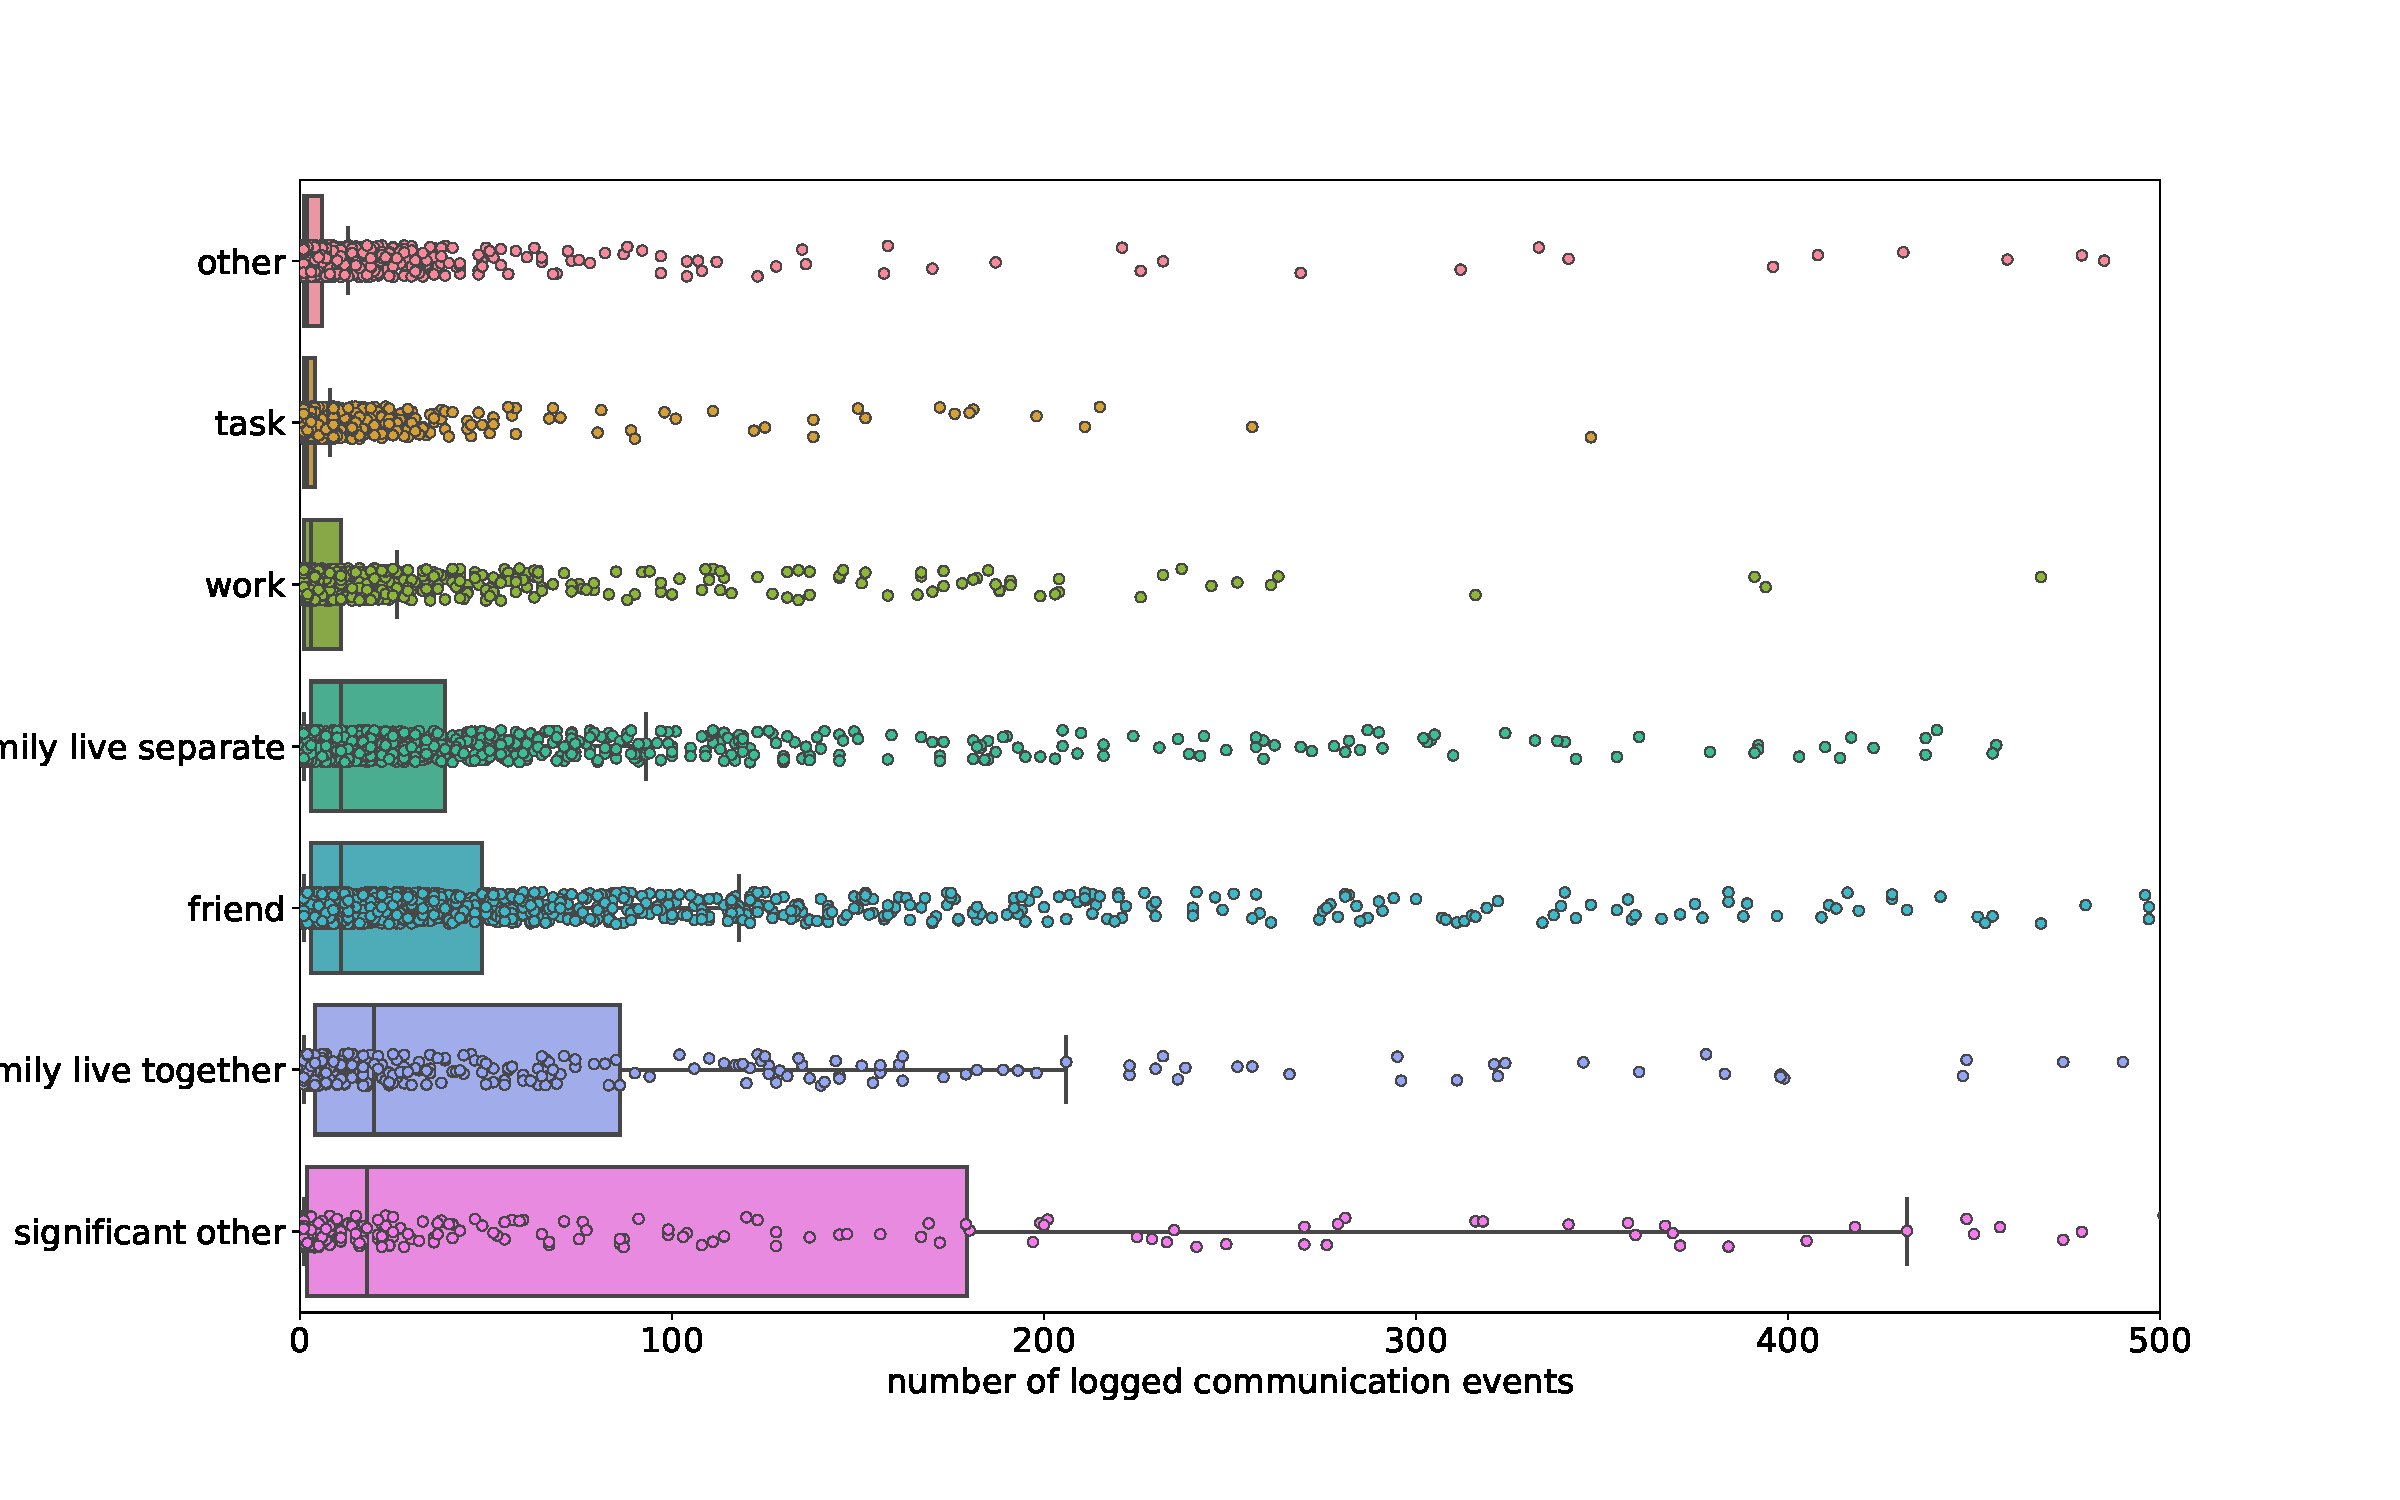
\includegraphics[width=1\textwidth]{figures/all_contact_types_comm_freq_strip.pdf}
    %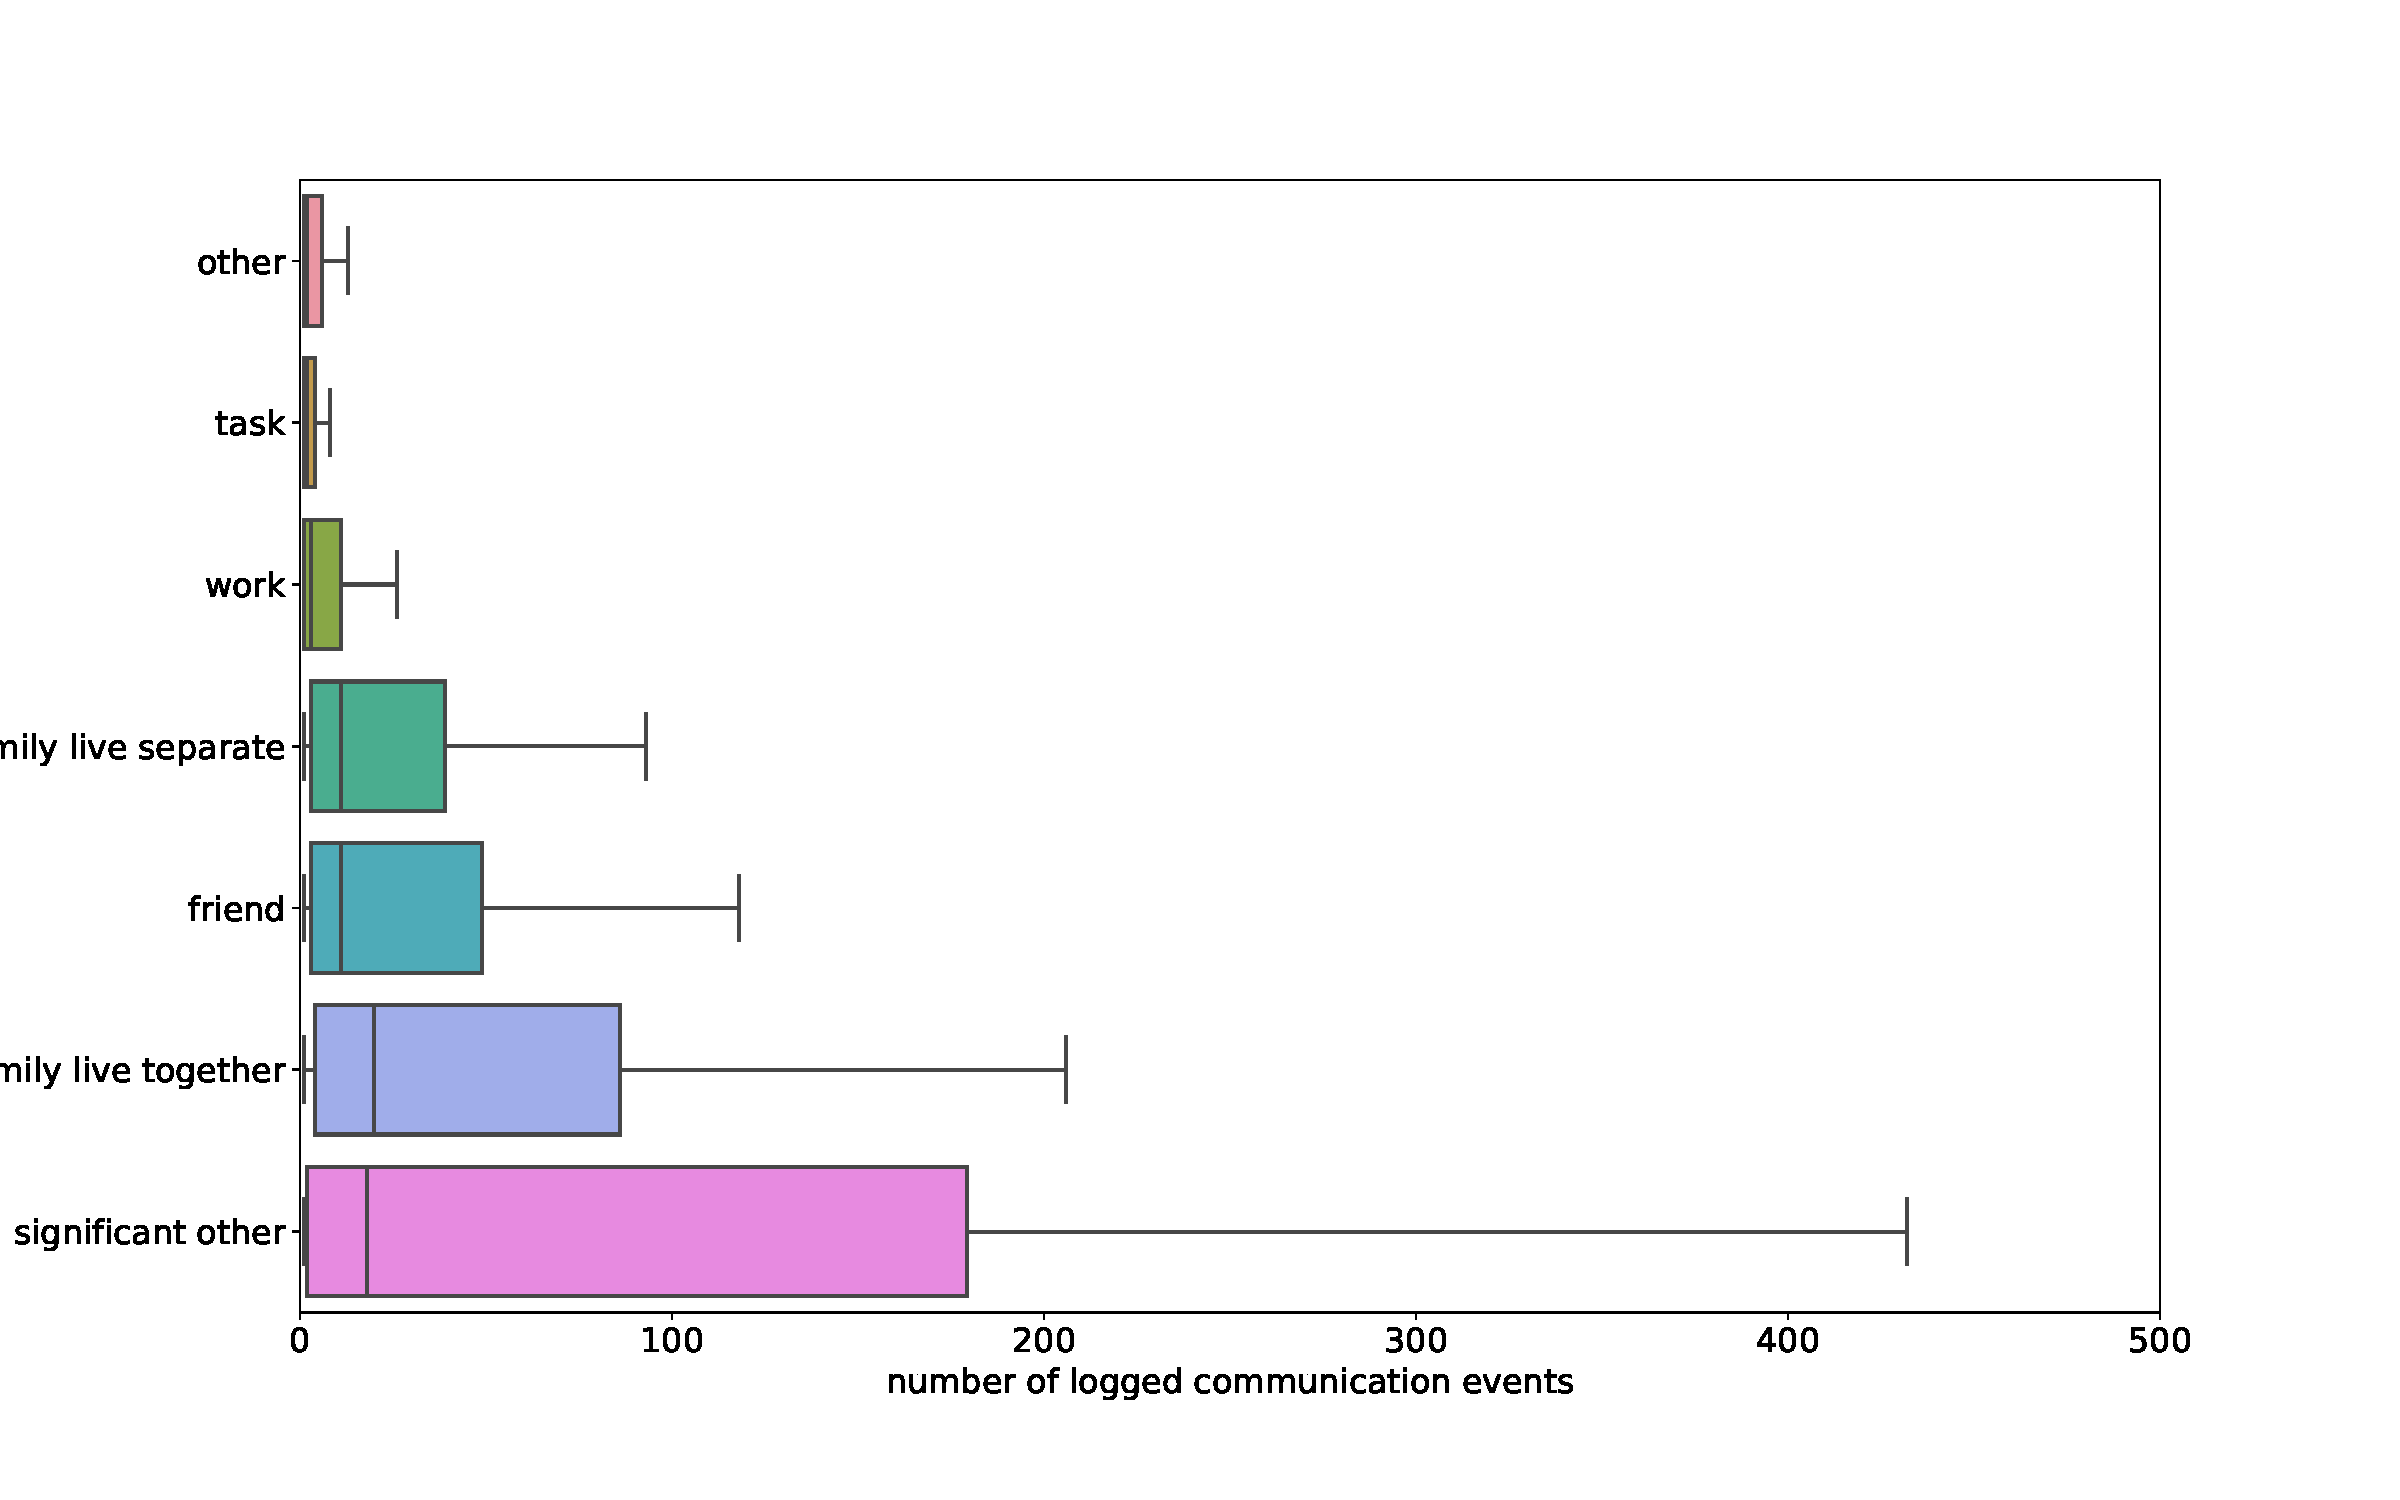
\includegraphics[width=1\textwidth]{figures/all_contact_types_comm_freq.pdf}
    \caption{\textbf{The relationship between contact type and communication frequency across all contacts}. Points overlaid on the box plots are individual contacts in our data. When considering all participants' contacts, we see that the vast majority of ``other'' and ``task'' contacts have few logged communication events, illustrating the need for a communication frequency cutoff to model the contacts that truly provide social support for their corresponding participant.}
    \label{fig:comm_frequency}
\end{figure}



% Motivation for collapsing classes
% \begin{itemize}
%     \item we examined the full 6-class prediction task, and noticed that FLS, F contacts were confused
%     spatial locality could play a role
%     \item we hypothesized that our models, in addition to estimating relationship types, also detect structure in spatial locality of contacts
%     % can make a point about semantic location analysis, but how does this move us towards the age argument?
%     \item to this end, we collapse labels to social ``separate'' and family ``living together'' classes and present our analysis on this four-class prediciton class
%     \item note that the six class results can be found in the supplemental section
% \end{itemize}

%In order to evaluate the strength of social ties to contacts, we generate a single \textit{tie strength} score by summing the EMA survey responses for each contact.  The range of possible values for tie strength are $0 - 24$, corresponding to the seven-point Likert scale used for the four survey questions. Following the reasoning presented in Wiese et al. for tie strength classification, we also analyze relative rankings of contact's tie strength scores per participant and partition tie strength into three classes: \textit{strong ties} (rank 1-4), \textit{medium ties} (rank 5-19), and \textit{weak ties} (rank 20 - ), corresponding to ``support'' groups, ``sympathy'' groups, and others, respectively~\cite{wiese2015you, zhou2005discrete}. The distribution of tie strength scores in our dataset roughly corroborate these categories (Figure~\ref{fig:tie_str_rank}): we see tie strength decrease at a constant rate through the strong and weak tie contacts, levelling off around the medium tie cutoff rank of 19.

% \begin{figure}
%     \centering
%     \includegraphics[width=0.5\textwidth]{figures/tie_str_rank.png}
%     \caption{Mean tie strength scores as a function of contact ranking per participant. Lighter regions indicate standard errors.}
%     \label{fig:tie_str_rank}
% \end{figure}

\subsection{Feature extraction}
\label{subsec:feature_extract}
For our prediction tasks, we consider a number of feature blocks: communication, demographics, and semantic location.

\subsubsection*{Communication features}

We derive 147 communication features based on previous work by~\cite{min2013mining}, replicating all of their features except for those relating to SMS length. These features fall into four broad categories as defined in~\cite{wiese2015you} and others:

% TODO elaborate on the broad categories
\begin{itemize}
    \itemsep0em
    \item \textit{intensity and regularity}: features that consider the volume and regularity of communication, such as mean or median weekly calls or number of study days with a logged communication.
    \item \textit{temporal tendency}: features that capture the time of day or day of week when communication events typically occur.
    \item \textit{channel selection and avoidance}: features that capture any asymmetry in communication (incoming vs. outgoing) or preference for calls vs. SMS.
    \item \textit{maintenance cost}: features that consider the amount of effort in maintaining communication relationships.
\end{itemize}

% TODO remove hyperlinks for paper submission
A full description of these features as well as summary statistics can be found at our project's Github page (Figure~\ref{fig:comm_features}).

%\href{https://github.com/tliu526/relationship-prediction/blob/master/feature_extract/feature_extract.ipynb}{Github page}



\subsubsection*{Demographic features}

Demographic information about each participant were treated as a separate feature block. This included age, gender, race, ethnicity, education, marital status, employment status, and whether the participant lived alone or with others. All of the categorical responses were encoded in a one-hot representation. Summary statistics of our participant demographics can be found in Table TODO.

\subsubsection*{Semantic location features}

To convert the raw GPS data into higher-level features, we use the adaptive k-means clustering methodology presented in~\cite{saeb2017mobile}. First, GPS readings were clustered with a maximum radius of 100 meters. Clusters that had durations of fewer than 10 minutes were discarded to handle transient locations, such as when a participant was stuck in traffic. Participants then answered two questions about the detected location clusters: ``what kind of place is this?" and ``why did you visit this place''? Responses were chosen from pre-defined categories, with options such as ``home'' or ``nightlife spot'' for the place type and ``entertainment'' or ``errand'' for the visit reason. A full list of the possible survey responses can be found in the Appendix. % TODO add to appendix

We then cross-reference the duration of time each participant spent at a location with their communication logs, so that an individual call or text could be labelled as sent or received from a particular location (Figure~\ref{fig:semantic_location}). These counts are normalized over all communication events for each contact, giving us relative proportions of communication events that occur at a semantic location.

% TODO update with own styling
\begin{figure*}
    \centering
    \includegraphics[width=1\textwidth]{figures/semantic_loc.png}
    \caption{\textbf{Semantic location chart over the study period for a representative participant.} We see some regularity in the participant's visits to ``home'' and ``work'' locations. }
    \label{fig:semantic_location}
\end{figure*}

\subsubsection*{Missing Data Imputation}

Due to the passive nature of how phone sensor data are collected, missing data are commonplace and needs to be appropriately handled. Furthermore, it is often the case that data are not missing at random, and the presence or absence of a feature can provide information (eg, a lack of calls to a contact between 12 am and 4 am). To this end, we not only impute missing features with the sample population median but also include a new indicator feature for whether the data are missing. This allows us to capture any potential patterns in how data are missing, which could provide additional information to the predictive models.

\subsection{Predictive modeling and procedural setup}


\subsubsection*{Cross validation methodology}

Because there is shared information between contacts sourced from the same participant, it is critical that we cross-validate over participants as opposed to over contacts to ensure that there is no data leakage. Saeb et al demonstrate that improper cross validation not only incorrectly inflates performance metrics, but also fails to measure the generalization of a model on true out-of-sample data~\cite{saeb2016voodoo}. In the context of relationship prediction, contacts that are associated with a particular participant could have similar communication tendencies based on individual variation as well as identical demographics, which could bias our model's estimation by potentially learning to identify individual participants as opposed to actually learning the characteristics of relationship classes. To this end, we train our models using \textit{grouped} $K$-fold cross validation, where all the contacts $c \in C_i$ associated with a participant $i$ are included in a single fold and the $K$ folds are defined in terms of groups of participants $P_k$ (Equation~\ref{eq:group_cv}). This cross-validation methodology ensures that our models do not over-fit the training data, producing meaningful performance results.

% TODO should this be captioned?
\begin{equation}
    \label{eq:group_cv}
    % TODO which is more readable?
    % \mathcal{L} = \sum^K_{k=1} \Big [ \sum_{i \in P_k} \frac{1}{|C_i|} \sum_{c \in C_i} \mathbf{1}\{\hat{y}_c \ne y_c\}\Big ]
    \mathcal{L} = \sum^K_{k=1} \Big [ \sum_{i \in P_k} \frac{\sum_{c \in C_i} \mathbf{1}\{\hat{y}_c \ne y_c\}}{|C_i|} \Big ]
\end{equation}

\subsubsection*{Automated machine learning}

% TODO CCC
We utilize \textit{auto-sklearn}~\cite{feurer2015efficient} for our feature selection, model selection, and hyperparameter tuning process. Model building occurs in three stages. First, a meta-learning step selects promising initializations of hyperparameters based on the given data's similarity to existing data. Next, specific algorithms and hyperparameter settings are tuned through Bayesian optimization~\cite{brochu2010tutorial}. Finally, the best models found through this optimization process are used to automatically construct an ensemble model, which is the final model output. Automatic selection of model parameters and ensembling not only tends to give slightly higher performance than manually engineering them, it also prevents any user bias from being introduced into the resulting model, such as a preference for one algorithm over another or prior knowledge about the dataset that can be exploited. Auto-sklearn is feature and algorithm agnostic, allowing us to essentially treat the model building process as a hands-off task.

% TODO add back repository information after review process
% Details on our exact auto-sklearn settings can be found in our Github repository.

\subsubsection*{Feature importance analysis using SHAP}

We not only want a model with good performance --- we would also like to interpret the relative importance of features when it makes predictions. However, because auto-sklearn builds ensembles of various machine learning models for its final output, feature weights are not directly accessible. Our solution is to use \textit{SHAP}, which combines numerous additive feature attribution techniques to produce a single ``explanation model''~\cite{lundberg2017unified}. The intuition behind these methods is that they map the original features of a local data point $x$ to a simplified space where the mapped inputs contribute additively to a linear explanation model describing the actual classifier output for $x$. These features can then be easily assigned importance based on their contributions to the explanation model. By using SHAP, we are able to give more intuitive analyses of our models' performance despite their complexity.

\section{Results: Relationship Prediction Analysis}
\label{sec:rel_pred_results}

To make progress at relationship prediction we need to choose the features and an evaluation procedure. We use the following feature sets: 
\begin{itemize}
    \itemsep0em
    \item age and gender
    \item communication features
    \item communication + age/gender features 
    \item communication + demographics + semantic location features
\end{itemize}
We hold out 25\% of the participants as an out-of-sample test set, and use accuracy, weighted F1 and macro F1 to evaluate final model performance. Random forests trained using the auto-sklearn framework serve as a baseline comparison to the auto-sklearn ensemble methods. These choices enable us to quantify relationship prediction as a function of the type of the feature set.

\subsection{Four-class Relationship Prediction Performance}
% TODO correct term for peer family members?
% TODO we'll likely need to justify more why we chose to collapse classes
For a meaningful comparison across relationship roles we must have classes that are sufficiently distinct. We first trained our models for relationship prediction utilizing all six relationship categories: ``family live together,'' ``family live separate,'' ``friend,'' ``work,'' and ``task.'' In these initial runs, we found that ``family live separate'' and ``friend'' contacts are often confused. We hypothesize that instead of predicting the social role, our models were detecting the structure of the relationship in whether the participant lives with the contact or not. This could have more impact on when and how participants communicate with contacts than any familial labels: communication patterns between ``peer'' family members who live separately such as siblings can bear closer resemblance to social relationships than other familial relationships. To this end, we define new labels where the  ``family live separate'' and ``friends'' labels are collapsed into a single category: ``social separate,'' and ``significant other'' and ``family live together'' labels are collapsed into a single category: ``family together.'' We note that the six-class prediction class results show similar trends in performance across the blocks of features, which can be found in Supplemental Figure~\ref{tab:top5_6class_metrics} and Supplemental Table~\ref{tab:top5_6class_metrics}. For the rest of our paper we thus focus on the four-class prediction task for model evaluation. 

% ommitting 6-class results to focus paper

\begin{table}[h!]
    \centering
        \begin{tabular}{llcccc}
        \toprule
                     model &    features &  accuracy &  macro f1 &  weighted f1 \\
        \midrule
         majority baseline &         N/A &    0.5714  &    0.1818 &       0.4156 \\
         \midrule
            random forest & age/gender & 0.5714 &    0.1818 &       0.4156 \\
             random forest &    comm &    0.6667 &    0.4795 &       0.6254 \\
             random forest &  comm + age/gender &    0.6667 &    0.4750 &       0.6225 \\
    %         Random forest &        demo &    0.6667 &    0.4598 &       0.6213 \\
             random forest & comm + demo + loc &    0.6762 &    0.4744 &       0.6326 \\
        \midrule
                    auto-sklearn & age/gender & 0.5714 &    0.1818 &       0.4156 \\
                    auto-sklearn & comm &    0.6571 &    0.4731 &       0.6195 \\
                    auto-sklearn &  comm + age/gender &    0.6905 &    0.5488 &       0.6654 \\
    %                auto-sklearn &        demo &    \textbf{0.7095} &             \textbf{0.5344} &    \textbf{0.5598} &       0.6775 \\
                    auto-sklearn & comm + demo + loc &    \textbf{0.7095} &    \textbf{0.5519} &       \textbf{0.6806} \\
        \bottomrule
        \end{tabular}

        \caption{\textbf{Performance metrics for the four-class relationship prediction task.} We show the highest scores in bold. Auto-sklearn is used for hyperparameter selection of the ``random forest'' models, while the ``auto-sklearn'' models are ensembles of the best performing models found via auto-sklearn's optimization process. Feature blocks correspond to the four feature configurations described above, with ``comm'' as communication features, ``demo'' as all demographic features, and ``loc'' as semantic location features. }
        \label{tab:top5_4class_metrics}
\end{table}

Our goal is to measure any improvement in relationship prediction when adding demographics and location features. Indeed, we find that including these features help model performance (Table~\ref{tab:top5_4class_metrics}). First, we note that due to class imbalance across our data the trivial strategy of always guessing the majority baseline (``social separate'') in fact sets a meaningful lower bound of performance to compare against. Our best performing model, the auto-sklearn ensemble trained with all of our features, achieves an accuracy of 71\% on the held-out test set, a 14 point increase in raw accuracy over the majority baseline prediction. Improvements over baseline are larger in the F1 scores with the ensemble model producing a macro F1 of 0.55 and a weighted F1 of 0.68. Across all metric comparisons we find that adding demographics and location features considerably improves prediction performance.

% TODO paragraph on auto-sklearn comparison
%A general trend we note is that the auto-sklearn ensemble models perform slightly better than the tuned random forest models, especially when trained with more features.

%TODO how to better conclude confusion matrix discussion? Doesn't quite fit with the feature analysis motivation. 
When evaluating performance, it is important for us to also consider misclassified contacts as they can provide information on the relationship between our contact types. We find that the across all types, the most common confusion is incorrectly predicting ``social separate'' (Table~\ref{tab:top5_4class_confusion}), which is not surprising given the class imbalance we have noted. Despite this, classification performance of ``task'' and ``family together'' labels is reasonable with accuracies of about 60\%. On the other hand, ``work'' contacts are almost entirely misclassified as ``social separate'' contacts. We hypothesize that given we only consider the top five contacts of each participants, contacts nominally labelled ``work'' are in fact contacts the participant is closer to, akin to a friend. This motivates the need to consider finer-grained contact types or alternative measures of social roles as contact type labels sometimes do not capture the complete context of a social relationship.

\begin{table}[h]
    \centering
        \begin{tabular}{lcccc}
        \toprule
        {} &  pW &  pSS &  pT &  pFT \\
        \midrule
        W            &       1 &        15 &       0 &                  0 \\
        SS          &       0 &       106 &       1 &                 13 \\
        T            &       0 &         7 &      11 &                  1 \\
        FT &       0 &        23 &       1 &                 31 \\
        \bottomrule
        \end{tabular}
        \caption{\textbf{Test set confusion matrix for the ``auto-sklearn'' ensemble model with all features.} Contact types are abbreviated work (W), social separate (SS), task (T), and family together (FT), and  columns, marked by ``p,'' are predictions.}
        \label{tab:top5_4class_confusion}
\end{table}

Breaking our model features into four separate configurations also allow us to examine relative changes in performance when introducing particular features. Across the ``auto-sklearn'' feature blocks (Table~\ref{tab:top5_4class_metrics}), we see the largest increase in performance when adding age and gender to our model with a 3.4\% bump in accuracy and 4.5 point increase in weighted F1, while including other demographics and location features on top of age and gender provide much smaller performance improvements. This increase when introducing age and gender features is particularly interesting when we consider the fact that age and gender features alone do not appear to have any predictive value: as shown in Table~\ref{tab:top5_4class_metrics}, models trained using only those features do no better than simply guessing the majority class. This is an indication that there is a potential interaction effect between age/gender and the other features, particularly communication features, that leads to the improvement in performance.

% \begin{table}[]
%     \centering
%         \begin{tabular}{llcccc}
%         \toprule
%                      model &    features &  accuracy &  balanced accuracy &  macro f1 &  weighted f1 \\
%         \midrule
%          majority baseline &         N/A &    0.5714 &             0.2500 &    0.1818 &       0.4156 \\
%          \midrule
%              Random forest &    comm &    0.6667 &             0.4590 &    0.4795 &       0.6254 \\
%              Random forest &  comm + age/gender &    0.6667 &             0.4566 &    0.4750 &       0.6225 \\
%     %         Random forest &        demo &    0.6667 &             0.4369 &    0.4598 &       0.6213 \\
%              Random forest & comm + demo + loc &    0.6762 &             0.4546 &    0.4744 &       0.6326 \\
%         \midrule
%                     auto-sklearn & age/gender & 0.5714 &             0.2500 &    0.1818 &       0.4156 \\
%                     auto-sklearn & comm &    0.6571 &             0.4598 &    0.4731 &       0.6195 \\
%                     auto-sklearn &  comm + age/gender &    0.6905 &             \textbf{0.5310} &    0.5488 &       0.6654 \\
%     %                auto-sklearn &        demo &    \textbf{0.7095} &             \textbf{0.5344} &    \textbf{0.5598} &       0.6775 \\
%                     auto-sklearn & comm + demo + loc &    \textbf{0.7095} &             0.5221 &    \textbf{0.5519} &       \textbf{0.6806} \\
%         \bottomrule
%         \end{tabular}

%         \caption{Performance metrics for the 4 class relationship prediction task with highest scores in bold. Feature blocks correspond to the configurations described above, with ``comm'' as communication features, ``demo'' as all demographic features, and ``loc'' as semantic location features.}
%         \label{tab:top5_4class_metrics}
% \end{table}


\subsection{Feature Importance}

Now that we have seen that the addition of demographic and semantic location features improve model performance, we wish to explore feature interactions with the various contact types as well as gain insight on their fine-grained effects on relationship prediction performance. To accomplish this, we use the SHAP framework to examine predictive feature importance across both individual features and our pre-defined feature blocks. Our analysis provides a degree of explanation as to why our models made their predictions and also sheds some light on specific communication patterns that characterize particular contact types.

%\subsubsection*{SHAP feature analysis}


% point 1: communication features are still the most important

% point 2: specifically, temporal tendency and intensity and regularity features


% point 3: semantic location

We know from our feature block setup that communication features are critical for good performance (Table~\ref{tab:top5_4class_metrics}), but we would like to gain some insight on features are actually contributing to model predictions for particular contact types. By examining the average SHAP magnitude, we see that that all but two of the top fifteen most important features are derived from communication patterns( Figure~\ref{fig:top5_ag_shap}), which is expected given the modest increases in performance when comparing the models trained with only communication features to our models with additional demographic and location features. Out of the four categories of communication features we construct (Section~\ref{subsec:feature_extract}), \textit{intensity and regularity} (total communication days, call duration, communication regularity) and \textit{temporal tendency} (communications made between 8pm and 12am, 12am and 4 am, and Sunday communications) are particularly prominent. The most important individual feature, total number of days of communication, is a strong signal for the ``family together'' and ``social separate, '' which is an intuitive relationship as this feature encapsulates both the regularity and volume of communication.  Through SHAP analysis of our features, we are able to see that the timing as well as the volume of communication are the most important factors in determining the nature of relationships participants have with close contacts.

% TODO paragraph of analysis for work and task contact types
% Work: Monday, and 8am - 12 pm texts
% Task: total number of communications and missed to incoming call ratio
The features that contribute to a ``work'' classification are texts on Mondays and calls between 8 am and 12 pm, again a reasonable relationship as communications during those time periods would seem to be indicative of work-related interactions.

Furthermore, this analysis highlights the contributions of certain semantic location features to our model outputs. We see that calls taken at locations where the the visit reason was ``errand'' and calls taken at shops are important (Figure ~\ref{fig:top5_ag_shap}). These two features make the largest contributions to the ``family together'' class output, a sensible result as communications while running errands or shopping (eg for groceries in a common household) will likely be made to contacts that live with the participant. This analysis demonstrates the value in including semantic location features as it can further contextualize communication events for particular contact types.

Notably absent in the top SHAP values however are demographic features, particularly age and gender. We hypothesize that there is an interaction effect...

\begin{figure}[h]
    \centering
    \includegraphics[width=0.8\textwidth]{figures/top5_all_shap.pdf}
    \caption{\textbf{Top 15 features of the best performing auto-sklearn model ordered by average SHAP value magnitude.} We see that features related to communication volume, regularity, and temporality are important. }
    \label{fig:top5_ag_shap}    
\end{figure}

%Now that we have seen that the addition of demographic and semantic location features improve model performance, we wish to examine individual features in order to gain insight on their fine-grained effects on relationship prediction. Here, we conduct both a correlation analysis to explore the interactions of our features with our contact type classes as well as predictive feature importance to examine effects on overall classification performance.

%\subsubsection*{Feature correlations}

%FDR reference~\cite{benjamini1995fdr}

%For performance analysis on our baseline random forest models we use the \textit{scikit-learn}~\cite{pedregosa2011scikit} implementation of \textit{gini importance}~\cite{breiman2017classification}, which is a calculation of the total decrease in node impurity for feature over all the trees in the random forest ensemble. For auto-sklearn model analysis, we use \textit{SHAP}~\cite{lundberg2017unified}, a unification of various additive feature importance measures. SHAP values are computed over our held-out test set.

%\subsubsection*{Random forest feature importance}

%TODO slide 20
% \begin{itemize}
%     \item though not the exact same features are selected, largely corroborates what SHAP shows
% \end{itemize}

\subsection{Age Interaction with Communication Patterns}

\begin{table}[h]
    \centering
    \begin{tabular}{lrr}
    \toprule
    communication features &   corr &     p \\
    \midrule
    call tendency                             &  0.181 & <0.001 \\
    12am - 4am communication                  & -0.146 & <0.001 \\
    12am - 4am SMS                            & -0.145 & <0.001 \\
    8pm - 12am SMS                            & -0.141 & <0.001 \\
    texting regularity                        & -0.139 & <0.001 \\
    Sunday SMS                                & -0.132 & <0.001 \\
    total \# texting days                     & -0.131 & <0.001 \\
    communication within last 2 weeks         &  0.129 & 0.001 \\
    Sunday communication                      & -0.128 & 0.001 \\
    Max incoming SMS frequency                & -0.118 & 0.002 \\
    8pm - 12am communication                  & -0.116 & 0.002 \\
    standard deviation incoming SMS frequency & -0.111 & 0.004 \\
    call duration within last 2 weeks         &  0.110 & 0.005 \\
    mean incoming SMS frequency               & -0.110 & 0.005 \\
    median incoming SMS frequency             & -0.108 & 0.006 \\
    median outgoing SMS frequency             & -0.107 & 0.006 \\
    SMS frequency within last 2 weeks         & -0.103 & 0.009 \\
    Max outgoing SMS frequency                & -0.103 & 0.009 \\
    \bottomrule
    \end{tabular}
    \caption{\textbf{Participant age correlations with communication features.} We show significant features with a false discovery rate of <0.01~\cite{benjamini1995fdr}, sorted by correlation magnitude.}
    \label{tab:age_comm_corr}
\end{table}



\section{Results: Subgroup Generalization Task}
\label{sec:subgroup_results}

 Many studies in the personal sensing and relationship prediction literature utilize student samples which are skewed towards younger age demographics, raising questions about their generalizability. We have shown in the previous section that participants of different ages have distinct communication patterns, which will likely impact relationship prediction model performance when applied to out-of-sample populations. To quantify this effect, we conduct a prediction task where we split our data into quartiles by age, train models within each quartile, and evaluate performance on the other quartiles. In order to have consistent comparisons across our relationship prediction tasks, we mirror the best-performing setup on our original relationship prediction tasks presented in Section~\ref{sec:rel_pred_results} by utilizing auto-sklearn with all of our derived features (communication, demographics, semantic location) and the same within-participant cross-validation procedure to train models on our four quartile subgroups. This across-group prediction task allows us to measure how age homogeneity may affect generalization.
 
 %To quantify the effect of homogeneous training samples on out-of-sample model performance, we split our data into quartiles by age, train models within each quartile, and evaluate model performance on the other quartiles. Conducting this across-group prediction task allows us to measure how age homogeneity may affect generalization. 

\subsection{Subgroup Data Description and Setup}

% TODO drop in correlation analysis across groups?
We need to understand the composition of each of our subgroup populations in order to ensure our prediction task properly evaluates model generalizbility. We initially considered a subdivision where groups were constructed based on whether participants were students, however we lacked the requisite sample size for a meaningful comparison across these groups. We also considered specific age cut-offs (eg participants under the age of 25), but decided that quartile boundaries set according to our data distribution would be the cleanest experimental setup for defining subgroups. The first quartile spans 18 to 31 year-olds and contains 52 participants, the second quartile spans 32 to 37 year-olds and contains 43 participants, the third quartile spans 38 to 46 year-olds, and the fourth quartile spans 47 to 66 year-olds (Figure~\ref{fig:subpop_age_hist}). We note that the number of participants and thus contacts are roughly the same in each quartile, so none of the models will have an undue advantage in training set size. Overall, we find that the quartile subgroup splits provide a clean methodology for evaluating relative model performance across different populations.

\begin{figure}
    \centering
    \includegraphics[width=0.75\textwidth]{figures/q_age_hist.png}
    \caption{\textbf{Histogram of participant ages with quartile cutoffs.} As defined by the distribution of participant ages in our sample, the cutoffs are defined at age 31 (Q1 to Q2), 37 (Q2 to Q3), and 46 (Q3 to Q4).}
    \label{fig:subpop_age_hist}    
\end{figure}

\begin{table}[]
    \centering
        \begin{tabular}{lrrrr}
        \toprule
        {} &  family together &  social separate &   task &  work \\
        \midrule
        Q1 &           20.38\% &           67.31\% &  5.00\% & 7.31\% \\
        Q2 &           25.58\% &           56.74\% & 10.70\% & 6.98\% \\
        Q3 &           24.71\% &           58.43\% &  8.63\% & 8.24\% \\
        Q4 &           21.86\% &           56.74\% & 12.09\% & 9.30\% \\
        \bottomrule
        \end{tabular}
    \caption{\textbf{Percentage of relationship labels within each age quartile.} Distributions are approximately equal across Q2, Q3, and Q4, while Q1 has roughly 10\% more ``social separate'' contacts.}
    \label{tab:subpop_contact_types}
\end{table}

Understanding the distribution of contact types within each group is also important when examining subgroup model performance. We see that though the proportion of each contact type is approximately the same across Q2, Q3, and Q4, Q1 has a larger amount of ``social separate'' labels when compared to the other quartiles (Table~\ref{tab:subpop_contact_types}). To address these relative differences between the proportion of contact types per quartile, labels are resampled so that all classes are equally represented in each cross-validation fold of the training procedure. Additionally, we choose to use macro F1 as our target metric to account for the class imbalance across our quartile samples; by evaluating our models using macro F1, trained models cannot artificially achieve higher out-of-sample performance simply by predicting the majority class. We note that the weighted F1 metrics (Supplemental Table~\ref{tab:subpop_perf_weight}) produces qualitatively the same trends as our subsequent performance analysis that focus on macro F1. These resampling and performance metric choices make the relative performances of each subgroup model more comparable.

% Here, we see that there are differences this distribution per quartile that could potentially impact relative model performance. 

Analogous to our question regarding the limits of model generalizability when trained on homogeneous samples, we also hypothesize that models trained on \textit{heterogeneous} data are able to generalize better across a wider test set population. To this end, we include model runs where we sample twelve participants from each quartile (48 participants total) to produce a heterogeneous training set and evaluate out-of-sample performance on the rest of the data --- this ``allQ'' model result is calculated as the mean performance over ten such samples drawn. The ``allQ'' model configuration allows us to evaluate the impact of having more varied training data on out-of-sample model performance.

\subsection{Subgroup Model Performance}

% TODO would be cool to plot the cumulative feature importance of SMS vs call features as function of the quartiles -> hopefully see a decrease in importance of SMS features as we go to higher quartiles

% Macro F1 results support our story the best
% "We use macro F1 because it has high dynamic range -> class imbalance doesn't help it"

% Within sample performance, as indicated by italics, are obtained by 5-fold cross validation and provide a benchmark for the best performance that can be achieved for that particular subgroup.

Though we naturally expect lower out-of-sample performance for our subgroup-trained models, we are interested in trends in relative performance across our models that can give insight for the generalizability of particular age quartiles. Indeed, we see that the model trained on the Q1 subgroup generalizes particularly poorly across the other subgroups, producing the worst performance out of all other models for its out-of-sample test subgroups (Table~\ref{tab:subpop_perf_macro}). Additionally, the Q2, Q3, and Q4-trained models produce their respective lowest test performance values on the Q1 subgroup. This could be due to the differences in class label distribution of the Q1 subgroup in comparison to the others (Table~\ref{tab:subpop_contact_types}), though our resampling of the training data would mitigate this effect. This could also be due to differences in the distribution of features in the Q1: for example, we have already seen that younger people have higher texting regularity than older people, which could result in the model trained on only Q1 data to over-emphasize texting features, leading to poor out-of-sample performance when those features are not as indicative of relationship labels in the older subgroups. Regardless of the exact source of this discrepancy in performance, what we have seen is that the youngest quartile in our sample is fundamentally different in both feature and relationship label composition than the rest of our sample. 

Furthermore, this experiment also illustrates the benefits of having a heterogeneous training sample. Our ``allQ''-trained models (last row of Table~\ref{tab:subpop_perf_macro}) produce the best average test performance across all four quartiles, and in all subgroups except for Q4. Performance of the overall model is within a standard deviation of the in-sample performance. This result is not entirely surprising, as when given a training set with more variance, models should generalize better to out-of-sample data. Still, the superior performance of the ``allQ''-trained models when compared to the others that are trained on more homogeneous data emphasize the standard lessons of machine learning, namely that ML techniques are good at interpolation not extrapolation of data.

% TODO move to discussion
% and that 

\begin{table}[h]
    \centering
    \begin{tabular}{lllll}
    \toprule
    Model &  q1 macro f1 &  q2 macro f1 &  q3 macro f1 &  q4 macro f1 \\
    \midrule
    majority &        0.205 &        0.174 &        0.183 &        0.184 \\
    q1-trained model       &        \textit{0.418} &        0.315 &        0.386 &        0.349 \\
    q2-trained model       &        0.353 &        \textit{0.479} &        0.426 &        0.456 \\
    q3-trained model       &        0.312 &        0.450 &        \textit{0.483} &        0.443 \\
    q4-trained model       &        0.321 &        0.455 &        0.397 &        \textit{0.587} \\
    allq-trained model     &        0.388 $\pm$ 0.038 &        0.468 $\pm$ 0.021 &        0.425 $\pm$ 0.022 &        0.487 $\pm$ 0.041 \\
    \bottomrule
    \end{tabular}
    \caption{\textbf{Performance of models trained on different sample subgroups, optimizing for macro F1.} Each row corresponds to a model trained on the indicated age quartile. Within sample results are obtained by 5-fold cross validation, indicated by italics.
    All-quartile models are trained on an equal number of participants sampled from each quartile, with the sampling procedure conducted ten times to produce the final average performance and standard deviations indicated.}
    \label{tab:subpop_perf_macro}
\end{table}

% \begin{itemize}
% \item Subpopulation prediction: we need to train on the right subjects $\rightarrow$ Really get towards the standard lessons of ML, interpolation etc (Tables ~\ref{tab:subpop_perf_weight},~\ref{tab:subpop_perf_macro})
%     \begin{itemize}
%         \item hypothesis: people of different ages have fundamentally different communication patterns --- ``students aren't people''
%         \item subdivide our sample population into quartiles
%         \item train models on resampled data within each quartile to account for class imbalance
%         \item models trained on youngest subpopulation generalized the worst
%         \item point to macro F1 scores for how a more heterogeneous mix of samples improves performance
%     \end{itemize}
% \end{itemize}



% \begin{table}[H]
%     \begin{tabular}{lllll}
%     \toprule
%     Model &  q1 micro f1 &  q2 micro f1 &  q3 micro f1 &  q4 micro f1 \\
%     \midrule
%     majority &        0.655 &        0.561 &        0.600 &        0.574 \\
%     q1-trained model       &        \textit{0.700} &        0.600 &        0.600 &        0.586 \\
%     q2-trained model       &        0.700 &        \textit{0.646} &        0.631 &        0.605 \\
%     q3-trained model       &        0.692 &        0.651 &        \textit{0.643} &        0.651 \\
%     q4-trained model       &        0.665 &        0.628 &        0.671 &        \textit{0.656} \\
%     allq-trained model     &        0.683 $\pm$ 0.026 &        0.628 $\pm$ 0.019 &        0.600 $\pm$ 0.026 &        0.628 $\pm$ 0.041 \\
%     \bottomrule
%     \end{tabular}
%     \caption{Performance of models trained on different sample subgroups, optimizing for micro F1. Each row corresponds to a model trained on the indicated age quartile. Within sample results were obtained by 5-fold cross validation and are indicated by italics.
%     All-quartile models are trained on an equal number of participants sampled from each quartile, with the sampling procedure conducted ten times to produce the final average performance and standard deviations indicated.}
%     \label{tab:subpop_perf_micro}
% \end{table}



\section{Discussion}
\label{sec:discussion}

\begin{itemize}
    \item How we filled the gap
    \begin{itemize}
        \item Analysis of interaction between demographics/semantic location with communication, yielding improvement in model performance
        \item Demonstration of the limits of generalizability in personal sensing models, and an exploration of why the differences in performance across age groups occur
        \item Note the difference in performance across papers $\to$ emphasizes the point of generalization
    \end{itemize}
    \item Our limitations
    \begin{itemize}
        \item Though large for the community, we still have relatively small $n$ 
        \item We also have a biased sample of our own, skewed towards females
        \item Our choice of prediction task may be limited, only considering top 5 vs all contacts
    \end{itemize}
    \item Future work
    \begin{itemize}
        \item Exploration of population heterogeneity across mood disorders
        \item Incorporation of data provenance to predictive models
    \end{itemize}
    \item Wider impact
    \begin{itemize}
        \item Results highlight the promise of passive sensing: additional feature modalities increase performance and reveal insights into individual communication patterns
        \item Also illustrate how many predictive modeling studies must be taken with a grain of salt: generalization and overfitting are great concerns the community must be mindful about
        \item our results should motivate future studies to strongly consider collecting heterogeneous data
        \item homogeneity is everywhere: even if one is only interested in modeling students, ensuring that the samples comes from a varied sample (eg not all psychology or computer science majors) can improve out-of-sample model performance
    \end{itemize}
\end{itemize}

% How we filled the gap
% TODO discuss differences in performances between our model and others
% they have a more homogeneous sample, fewer class labels, and "easier" contacts (not top five)
We have explored the impact of utilizing demographic and semantic location information in addition to typical communication features on relationship prediction model performance. Observing the interaction between age demographics and communication patterns, we also have conducted an age subgroup model generalization experiment where we highlight both the limits of generalizability when training models on homogeneous samples as well as the benefits of training on heterogeneous ones. Our use of automatic machine techniques throughout these tasks limit manual intervention in the model building and prediction process, a practice that we believe will encourage a more standardized methodology for tackling machine learning problems. 

% significance of the inclusion of demographics and location features

% significance of our subgroup prediction task
% - young populations generalize poorly
Within our data, training on the youngest population produces particularly poor results, highlighting the need to consider a more varied sample when training and evaluating models especially given the large proportion of studies that rely on younger (eg student) populations in the personal sensing space. 
% - heterogeneous training data produce the best results
Furthermore, the ``allQ'' models that produce superior performance when training on more varied samples indicate that it would behoove studies that aim to evaluate their predictive model's effectiveness ``in the wild'' to collect heterogeneous data to train and test on.

% dedicated thought to the performance of auto-sklearn
Though auto-sklearn is clearly not a silver bullet to all machine learning problems, it does provide a reasonable benchmark of other models; significant performance gains above automatic methods likely exploit patterns in the data, which in the relatively small sample size regime of personal sensing could limit the generalizability of particular techniques.

% Our limitations
Our study has some limitations that we wish to highlight. Though our dataset is larger than what is typical within the community, our sample size is likely still inefficient to truly demonstrate applicability and robustness of models to a wider population. %TODO power calculation citation

% Future Work
We also see an opportunity in improving model performance where features are derived from disparate data sources, which is common in the personal sensing field. By placing all sensor modalities into a single feature table, we are losing information about data provenance: semantic locations are fundamentally different than communication frequency and should be treated and regularized accordingly, yet they are analyzed in a homogeneous block. Even subcategories such as our \textit{maintenance cost} and \textit{temporal tendency} communication features carry different semantic meanings which could be useful for model creation. Future work could see applications of feature blocking techniques such as group lasso to personal sensing tasks, given the heterogeneous feature modalities of passive sensing.

% Wider Impact
Though personal sensing models have shown promise in understanding interpersonal relationships, the robustness of such models need to be validated for wider populations.

\pagebreak
\appendix

\renewcommand\thefigure{\thesection.\arabic{table}}    
\setcounter{table}{0}

\renewcommand\thefigure{\thesection.\arabic{figure}}    
\setcounter{figure}{0}

\section{Supplemental Figures and Tables}

\begin{table}[h]
    \centering
    \begin{tabular}{llrrrr}
        \toprule
        model & features & accuracy &  balanced accuracy &  macro f1 &  weighted f1 \\
        \midrule
        majority baseline & N/A &   0.3381 &             0.1667 &    0.0842 &       0.1709 \\
        \midrule
         Random forest &  comm &  0.4000 &             0.2994 &    0.2899 &       0.3559 \\
         Random forest & comm + age/gender & 0.4476 &             0.3543 &    0.3627 &       0.4123 \\
%         Random forest & comm + demo &    0.4476 &             0.3330 &    0.3291 &       0.3905 \\
         Random forest & comm + demo + loc  & 0.4333 &             0.3733 &    0.3577 &       0.4106 \\
        \hline
        auto-sklearn  & comm & 0.4524 &             0.3617 &    0.3534 &       0.4113 \\
        auto-sklearn & comm + age/gender &  0.4619 &             0.4150 &    \textbf{0.4294} &       \textbf{0.4523} \\
%        auto-sklearn & comm + demo &  0.4571 &             0.3818 &    0.3926 &       0.4344 \\
        auto-sklearn & comm + demo + loc & \textbf{0.4619} &  \textbf{0.4178} &    0.4261 &       0.4517 \\
        \bottomrule
    \end{tabular}
    \caption{Performance metrics for the 6 class relationship prediction task with highest scores in bold. Feature blocks correspond to the configurations described above, with ``comm'' as communication features, ``demo'' as all demographic features, and ``loc'' as semantic location features.}
    \label{tab:top5_6class_metrics}
\end{table}

\begin{table}[h]
    \centering
    \begin{tabular}{|lrrrrrr|}
        \hline
        {} &  pW &  pF &  pT &  pFLS &  pFLT &  pSO \\
        \hline
        W   &    2 &    7 &    0 &      6 &      0 &     1 \\
        F   &    3 &   42 &    1 &     18 &      2 &     5 \\
        T   &    1 &    3 &   14 &      1 &      0 &     0 \\
        FLS &    0 &   21 &    0 &     20 &      4 &     4 \\
        FLT &    0 &    3 &    1 &      7 &      4 &     5 \\
        SO  &    0 &   10 &    1 &      7 &      2 &    15 \\
        \hline
        \end{tabular}
        \caption{Top 5 test set confusion matrix using auto-sklearn for work (W), friend (F), task (T), family live separate (FLS), family live together (FLT), and significant other (SO) classes. Columns, marked by ``p,'' are predictions.}
        \label{tab:top5_6class_confusion}
\end{table}

\begin{table}[h]
    \centering
    \begin{tabular}{lrrrr}
    \toprule
    Model &  q1 weighted f1 &  q2 weighted f1 &  q3 weighted f1 &  q4 weighted f1 \\
    \midrule
    majority               &           0.550 &           0.411 &           0.395 &           0.359 \\
    q1-trained model       &           \textit{0.640}   &           0.507 &           0.569 &           0.519 \\
    q2-trained model       &           0.642 &           \textit{0.635}   &           0.567 &           0.585 \\
    q3-trained model       &           0.658 &           0.648 &           \textit{0.634}   &           0.623 \\
    q4-trained model       &           0.633 &           0.597 &           0.610 &           \textit{0.617}   \\
    allq-trained model     &           0.643 $\pm 0.014$ &           0.610 $\pm 0.042$ &           0.574 $\pm 0.017$ &           0.585 $\pm 0.034$ \\
    \bottomrule
    \end{tabular}
    \caption{Performance of models trained on different sample subgroups, optimized for weighted F1. Each row corresponds to a model trained on the indicated age quartile. Within sample results were obtained by 5-fold cross validation and are indicated by italics.  All-quartile models are trained on an equal number of participants sampled from each quartile, with the sampling procedure conducted ten times to produce the final average performances.}
    \label{tab:subpop_perf_weight}
\end{table}[h]

\section{Additional feature information}

\begin{figure*}
    \centering
    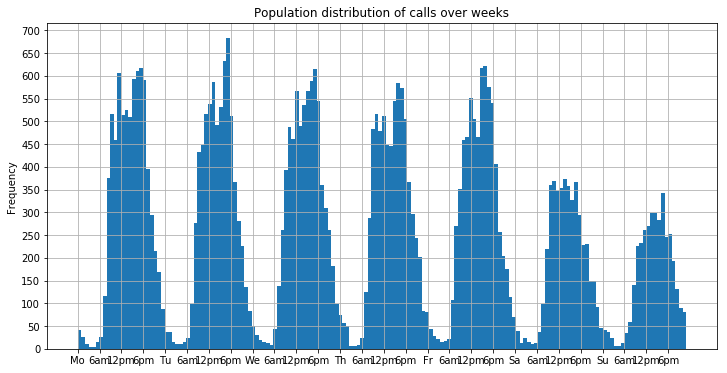
\includegraphics[width=0.8\textwidth]{figures/call_trend.png}
    \caption{Communication call patterns over days of the week. We see that there is an asymmetry between incoming/outgoing calls that is not present in SMS events.}
    \label{fig:comm_patterns}
\end{figure*}

\begin{figure*}
    \centering
    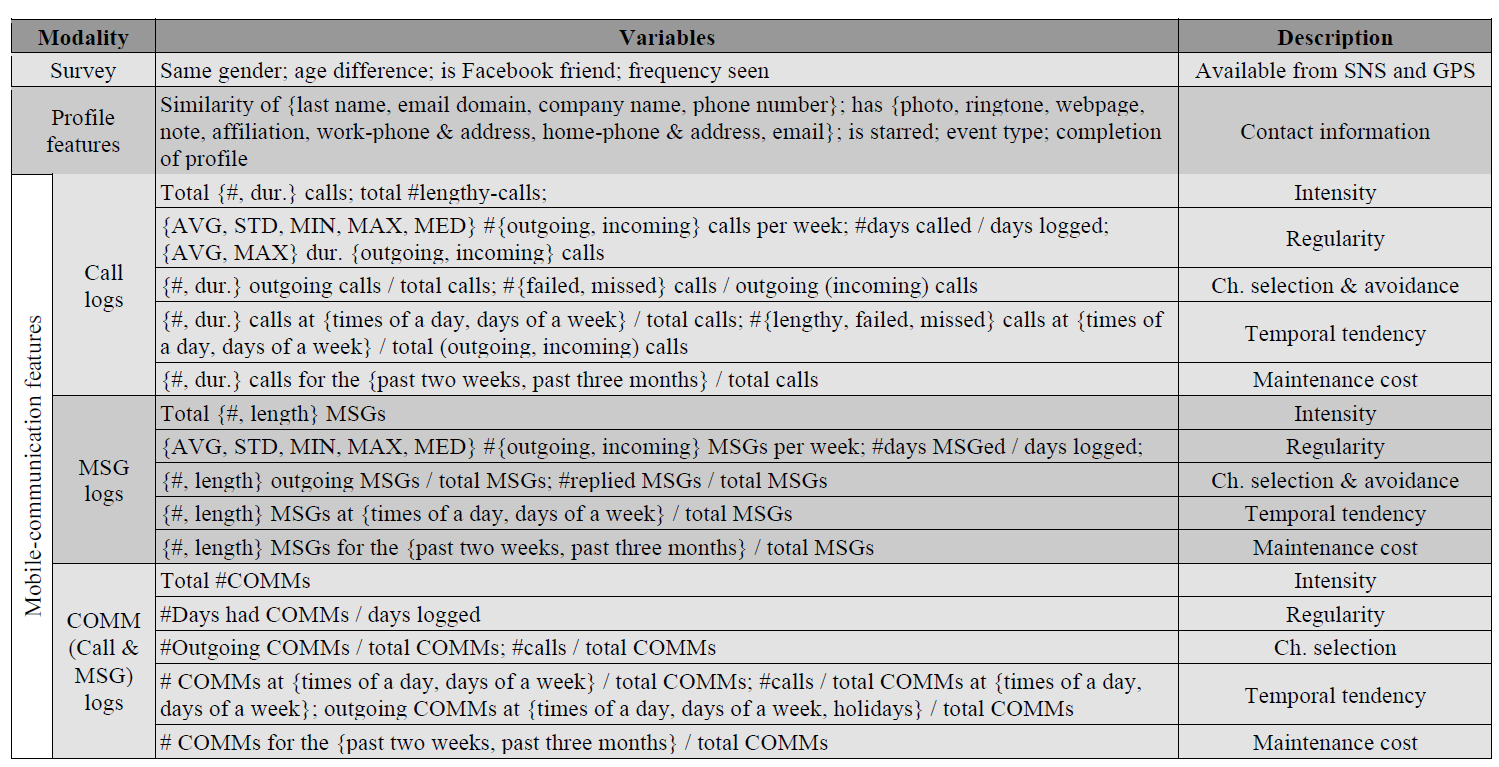
\includegraphics[width=1\textwidth]{figures/feature_extraction_placeholder.png}
    \caption{Table of extracted communication features, derived from~\cite{min2013mining}}.
    \label{fig:comm_features}
\end{figure*}

\pagebreak

\pagebreak

%\nocite{*} % for showing all references
\bibliographystyle{plain}
\bibliography{references}

\end{document}\documentclass[acmlarge]{acmart}
% alternate title: ML for Phone-Based Relationship Estimation: Considering Location Semantics and Population Heterogeneity
\title{Machine Learning for Phone-Based Relationship Estimation: The Need to Consider Population Heterogeneity}
\date{}
\author{}

% TODO have to make sure that the packages play nice with the latex template format
% \usepackage{amsmath}
% \usepackage{float}
% \usepackage[margin=1in]{geometry}
% \usepackage{graphicx}
\usepackage{hyperref}

%\usepackage[nomarkers, figuresonly]{endfloat}
% \usepackage[utf8]{inputenc}
% \usepackage{multicol}
%\usepackage{natbib}
%\usepackage{titlesec}
% \usepackage{xcolor}

%\titlespacing*{\section}{0pt}{0.5\baselineskip}{0.5\baselineskip}
%\titlespacing*{\subsection}{0pt}{0.5\baselineskip}{0.5\baselineskip}

\begin{abstract}
%IMWUT abstract length: 150-200 words
Estimating the category and quality of interpersonal relationships from ubiquitous phone sensor data matters for studying mental well-being and social support. Prior work focused on the volume of communications to estimate broad relationship categories. Here we contextualize communications by combining phone logs with demographic and location data to predict interpersonal relationship roles, producing better performance ($F1=0.68$) than using communication features alone. We also explore the effect of age variation in the underlying training sample on interpersonal relationship prediction and find that models trained on younger subgroups, which is popular in the field, generalize poorly to the wider population. Our results not only illustrate the value of using data across demographics, communication patterns and semantic locations, but also underscore the importance of considering population heterogeneity in phone-based personal sensing studies.
\end{abstract}

\begin{document}

\maketitle

\section{Introduction}
\label{sec:intro}
% Why care about estimating relationships?
Being able to understand the nature of interpersonal relationships and phone-based communication can be useful for studies of mental health. Studies have shown connections between perceived social support within relationships and effects of stress~\cite{cutrona1987provisions}, mood disorders such as depression~\cite{george1989social}, and psychological disorders such as schizophrenia and substance abuse~\cite{salyers2001social}. An individual's interpersonal context can be an indicator or risk factor: depressed individuals exhibit asymmetric communication patterns where they are less likely to initiate social interactions~\cite{hames2013interpersonal} while individuals with a strong support network are less prone to depressive episodes. The social role a specific contact plays is critical, as a call from work provides a vastly different kind of interaction and social support to an individual than a call from a friend. 

% Role/Advantages of passive-sensing
With the proliferation of smart mobile devices that passively collect data on user behavior~\cite{harari2017smartphone}, there is an increasing interest in estimating behavioral markers like social communication context through passive sensing~\cite{lane2010survey,mohr2017personal}. Automated analysis of such passive data can potentially provide avenues for early detection of mental health~\cite{canzian2015trajectories}. If an automated process could detect elevated risk factors for mental health in a person, that individual could be targeted for a more thorough assessment (and provided with digitized forms of support and treatment), alleviating many of the constraints associated with traditional assessment methods~\cite{suchman1962analysis}.

% Prior work and gaps
Previous works in passive sensing to estimate social relationships, tie strength, and friendship networks have used feature modalities such as communication logs, Bluetooth proximity, and geo-location tags to build machine learning models~\cite{eagle2009inferring,min2013mining,wiese2015you,hsieh2014inferring}. However, many of these studies focus on broad social categories (such as friend vs. not friend~\cite{eagle2009inferring}, and social vs family vs work~\cite{min2013mining}) where there could be overlap between roles or contacts that do not fit cleanly into a category. Moreover, we currently know little about the relationship of communication events with demographic and semantic location information, which could reveal additional fine-grained relationship information. We need to learn more about fine grained aspects of relationship and its generalization across demographics.

Furthermore, machine learning is not a cure-all, especially given the small sample sizes in the mobile personal sensing literature. Previous meta-analyses revealed that most papers utilize spurious baselines that lead to false optimism in the model results~\cite{demasi2017meaningless}. As machine learning tools become more ubiquitous and accessible, there is also a concern that methods are incorrectly applied. A literature review focusing on phone sensing models found that improper record-wise cross-validation which overestimates performance is frequently utilized in this space~\cite{saeb2016voodoo}. More generally, there is the issue of replication: studies are often conducted on a narrow group such as college students~\cite{eagle2006reality, wang2014studentlife} that may not generalize to a wider population~\cite{mohr2017personal}. Our goal is not just to produce good machine learning results but also to build generalizable models that are clinically and statistically meaningful.

% Our contributions
To address these gaps, we take a principled approach to social role prediction by contextualizing communication events with location and demographic data on a larger participant population ($n=187$) collected from across the United States. We make the following contributions:

\begin{itemize}
    \item We use \textit{auto-sklearn}, an automated machine learning technique~\cite{feurer2015efficient}, to build our models in order to reduce the biases introduced by manual model and feature selection.
    \item We contextualize participant's communication patterns with semantic location information and demographics, achieving a weighted F1 score of 0.68 on a held-out test set.
    % TODO more emphasis on age interactions
    \item We perform feature analysis and show that there are significant correlations between both the temporal tendency and channel selection of communication patterns and the age of the participants.
    \item We present an experiment where models are trained only on subsets of the population divided into age quartiles to illustrate the impact of population heterogeneity on model performance.
\end{itemize}

The rest of the paper is organized as follows. We review related work in Section~\ref{sec:related_work} and describe our data collection, feature extraction, and modeling methodology in Section~\ref{sec:methods}. In Section~\ref{sec:rel_pred_results}, we present our relationship prediction modeling results and analyze feature importance as well as correlations in communication patterns. We introduce our subgroup prediction task and subsequent performance analysis in Section~\ref{sec:subgroup_results}. We conclude by discussing implications of our results as well as limitations in Section~\ref{sec:discussion}.

\section{Related Work}
\label{sec:related_work}

% \textbf{Thread of gaps throughout related work}
% \begin{itemize}
%     \item small n studies with students for relationship prediction
%     \item focus on communication features and colocation information (symmetric relationships, not easily obtained), relatively little focus on semantic location which can be more easily obtained
% \end{itemize}

The ubiquity of personal sensing platforms has provided an opportunity for many novel modeling methods of human social behavior. In particular, there have been numerous previous studies for predicting relationship roles or social network analysis through passively collected phone data spanning different sensor modalities, such as bluetooth and communication logs. However, many of these studies also use data drawn from student or university participants, which are not representative samples of the wider population. We review prior work here to examine the breadth of model features as well as sample populations used in the literature.

% sample analysis of prior work: predominantly student populations 
Understanding the composition of the underlying sample population is important for the evaluation of a predictive model's generalizability. An influential work in estimating social systems using phone sensors, Reality Mining~\cite{eagle2006reality}, gathered bluetooth proximity, usage, and communication data from an academic population, where the 94 participants in the study were affiliated with MIT. Groups have used this public dataset to predict friend vs non-friend relationships with high accuracy through a variety of features such as spatial proximity~\cite{eagle2009inferring} and communication logs~\cite{mirisaee2010mining} as well as through novel modeling settings such as semi-supervised network inference~\cite{yu2017semi}. Numerous other works have leveraged student samples to produce effective relationship prediction models, albeit at small sample sizes~\cite{reinhardt2015show,hsieh2014inferring,dwarakanath2016analyzing}, and other similar works with different inference targets such as social support~\cite{ghosh2018modeling}, depression assessment~\cite{lu2018joint}, and happiness~\cite{jaques2015predicting} have also been extensively explored within students as well. Though academic populations are accessible for research groups, models trained on these data may not produce results that can ultimately generalize to other samples of differing demographics or even of different academic institutions.

% more heterogenous samples -> still not large or varied enough
Thus, in order to improve a model's efficacy across a general population more varied training samples are required. Indeed, there are other studies that have collected data from more heterogeneous populations: Min et al~\cite{min2013mining}'s study of predicting \textit{life facets} (family, work, social) from phone data as well as a follow-up study of tie strength~\cite{wiese2015you} use a sample of 40 participants recruited across the United States, though they are still majority students. Choi et al~\cite{choi2013mining} mine relationship types from 22 participants within a workplace environment, though their population is homogeneous in other aspects: 20 of the participants were male and all were computer science majors. The data used by the CommSense phone mining framework~\cite{bao2015commsense} crowd-source their sample of 106 users from geographically diverse areas in the United States. Overall however, a vast number of studies in the personal sensing space draw from small, homogeneous samples that are skewed towards a particular demographic.

% standard communication features and colocation data
% TODO not sure if highlighting shortcomings of co-location information buys us anything in the argument
Mobile devices today drive a significant amount of social interaction through digital communication, which is clearly important for determining the nature of social relationships. Consequently, the primary modeling features utilized across previous relationship prediction work are communication patterns extracted from text message, call, email, and instant message logs which are easily accessed through phone sensor data platforms~\cite{mirisaee2010mining,dwarakanath2016analyzing}. Co-location information is also often used to infer social network structure~\cite{eagle2009inferring,yu2017semi,hsieh2014inferring,choi2013mining}. However, co-location information requires ``symmetric'' data (from both target participants and their contacts) to be collected which would be more difficult to collect at scale or when participants are not spatially located in a similar geographic area. Part of the appeal of personal sensing is that data like communication logs are much easier to collect, making subsequent prediction models applicable to a wider range of source data and populations.

% additional demographic, and location features
Though phone communication patterns are good indicators for social relationships, differences in how users behave (eg due to life stage) or missing context (eg communications while traveling) potentially limit the predictive ability of communication features alone~\cite{wiese2015you}. Previous studies address this by leveraging other sensor modalities in addition to communication features to improve their models. Min et al include demographic information (age, gender differences) as well as survey results that capture additional relationship information such as closeness, finding that the combination of this information with communication fetures produced the best predictive performance~\cite{min2013mining}. The CommSense system uses basic semantic location information to contextualize communication events, with labels for calls or texts that occur at home or at work~\cite{bao2015commsense}. Overall however, inferring social relationships with other features such as demographics and location needs to be explored further, as these data are easily collected through personal sensing platforms and can better characterize communication patterns.

% how our study is unique: larger sample, heterogeneous population, semantic location information
% TODO feels a lot like a recapitulation of the contributions in the intro
Our work builds upon these existing studies by introducing fine-grained demographic and user-categorized location features for relationship prediction on a large, heterogeneous dataset. Though our location labels are more detailed than the high-level work vs home vs other categories used in CommSense, previous work by Saeb et al has demonstrated that semantic location can inferred from phone sensor data with good performance~\cite{saeb2017mobile}, making these features viable for use in other personal sensing studies. The addition of these feature blocks should not only improve predictive performance but also provide additional context as to how people interact with contacts of a particular relationship type.

We also make contributions from a modeling perspective by using automated machine learning methods~\cite{feurer2015efficient}. Lane et al note that most groups in the personal sensing space use hand-coded and hand-tuned models, which lead to questions on not how well these models generalize but also on how these models can be shared and standardized~\cite{lane2010survey}. Automated machine learning methods are powerful but also limit the user intervention when training and building predictive models, which could provide a common platform for the evaluation of various personal sensing tasks going forward.

Additionally, we note that the vast majority of these studies use small $n$ samples that are primarily drawn from student populations, which are often homogeneous demographically, particularly in terms of their age distribution. Our age-based subgroup experiment presented in Section~\ref{sec:subgroup_results} will explore the impact of training on such homogeneous samples, highlighting the need to collect data from more varied populations in order for personal sensing models to generalize.

\section{Methods and Data}
\label{sec:methods}
%The question we wish to answer is: can we predict contact communication roles and tie strength using passively collected phone features? We consider semantic location, demographics, and communication feature modalities as well as various target predictions: higher level three-class social role classification, finer-grained six-class social role classification, as well as classification and regression of contact tie strength. We leverage \textit{auto-sklearn} throughout all our experiment settings.

\subsection{Data Collection}
\label{subsec:data_collection}

% TODO elaborate on data collection methodology
Our dataset consists of 199 individuals (163 female, 33 male, 3 other) recruited between October 28, 2015 and February 12, 2016 across the United States that were at least 18 years old ($\mu = 38.27 \text{ yrs}, \sigma=10.19$), owned an Android smartphone (OS 4.4 through 5.1), and had access to WiFi. Individuals with psychotic disorders, inability to walk half a mile, or positive screens for alcohol abuse were excluded from our study. Participants were enrolled in the study for six weeks, where they installed \textit{Purple Robot}~\cite{purplerobot}, an open source Android application for recording phone sensor data, on their devices. 

% TODO flesh out with codebook information
\subsubsection*{Passive sensing}
Call and text information was logged, including whether the communication was incoming, outgoing, or missed as well as the total call duration. 

\subsubsection*{EMA and survey data}
In addition to the passive data collection, participants responded to EMA surveys that asked questions about semantic location as well as the contacts they communicate with. After the conclusion of the first logged communication, contacts were labelled with one of seven possible options:

\begin{itemize}
    \itemsep0em 
    \item Significant Other
    \item Friend
    \item Family Member You Live With
    \item Family Member You Don't Live With 
    \item Colleague/Work-Related
    \item Task (e.g. Make an Appointment, Reservation, etc.)
    \item Other
\end{itemize}

% Given that we're not focusing on tie strength for this paper, this should be omitted?
% Additionally, participants answered short questionnaires for each contact on a seven point Likert scale:

% \begin{itemize}
%     \itemsep0em 
%     \item How much did you want to communicate with this person today?
%     \item I would talk to this person about important matters
%     \item I would be willing to ask this person for a loan of \$100 or more.
%     \item How close are you to this contact?
% \end{itemize}

In total, for our participants we have 9,645 recorded contacts across 52,850 calls and 353,467 SMS messages. 
% TODO summarize basic distributions with a histogram, or ranked order plot
The number of contacts per participant is varied, with ranges from a single contact to 159 contacts (25th percentile: 24, 50th percentile: 37, 75th percentile: 58).

\subsection{Prediction Target: Top Five Contacts}
\label{subsec:target_categories}

\begin{table}[h]
    \centering
    \begin{tabular}{lcc} 
        \toprule
        {} & All contacts & Top 5 contacts \\
        \midrule
        family live separate & 1,232 & 249 \\
        family live together & 317 & 104 \\
        friend & 1,742 & 314 \\
        other & 1,939 & 87 \\
        significant other & 289 & 120\\
        task & 2,240 & 66 \\
        work & 1,189 & 73 \\
        \bottomrule
    \end{tabular}
    \caption{\textbf{Contact type counts for all contacts and top five contacts by communication frequency per participant.} When limiting to only top five contacts, classes that we expect to provide more social support are better represented, namely family members, friends, and significant others.}
    \label{tab:contact_types}
\end{table}

We examine the distribution of contacts types to ensure we have a well-defined prediction target for our relationship modeling task. When considering all contacts across our data, the most frequent contact types that occur are ``other'' followed by ``task'' (see ``all contacts'' column of Table~\ref{tab:contact_types}) which is likely due to a high volume of one-off communication events. Indeed, we see in Figure~\ref{fig:comm_frequency} that ``other'' and ``task'' contacts have much lower communication volume when compared to the other contact types. Consequently, we exclude ``other'' labels as a category in our prediction task due to the label being a catch-all for contacts that did not fit clearly into one of the predefined categories, which makes the classification task more meaningful.

In order to further focus the relationship modeling and to make the prediction target setup clean, we also restrict our data to each participant's top five contacts by communication volume, where ``friend'' and ``family live separate'' contact categories become the most frequent (see ``top 5 contacts'' column of  Table~\ref{tab:contact_types}). We choose this cutoff for a number of reasons. First, restricting the number of contacts per participant to a constant ensures that every participant is evenly represented in the data. Furthermore, removing the less frequent contacts from the data makes the prediction task non-trivial, as we can see given class imbalance of ``task'' labels (Table~\ref{tab:contact_types}) that a naive model could achieve good performance simply by considering the communication volume for contacts (Figure~\ref{fig:comm_frequency}). Finally, prior work in social grouping patterns indicate that individuals form small groups of three to five with others as \textit{social support}~\cite{dunbar1995social, zhou2005discrete}, making relationship role estimation of the top five contacts particularly important. With this choice of considering the ``top five'' contact types, we have defined a classification task that has a clean modeling setup and can also provide insight into the interactions between participants and their social support group. 


%We also note that our data lends itself to social ``tie strength'' estimation across contact types akin to the study presented by Wiese et al~\cite{wiese2015you}, which could be explored in future work.

%previous work has demonstrated that contacts with stronger ties are often more difficult to differentiate~\cite{wiese2015you}

\begin{figure}[h]
    \centering
    % TODO strip plot or normal boxplot?
    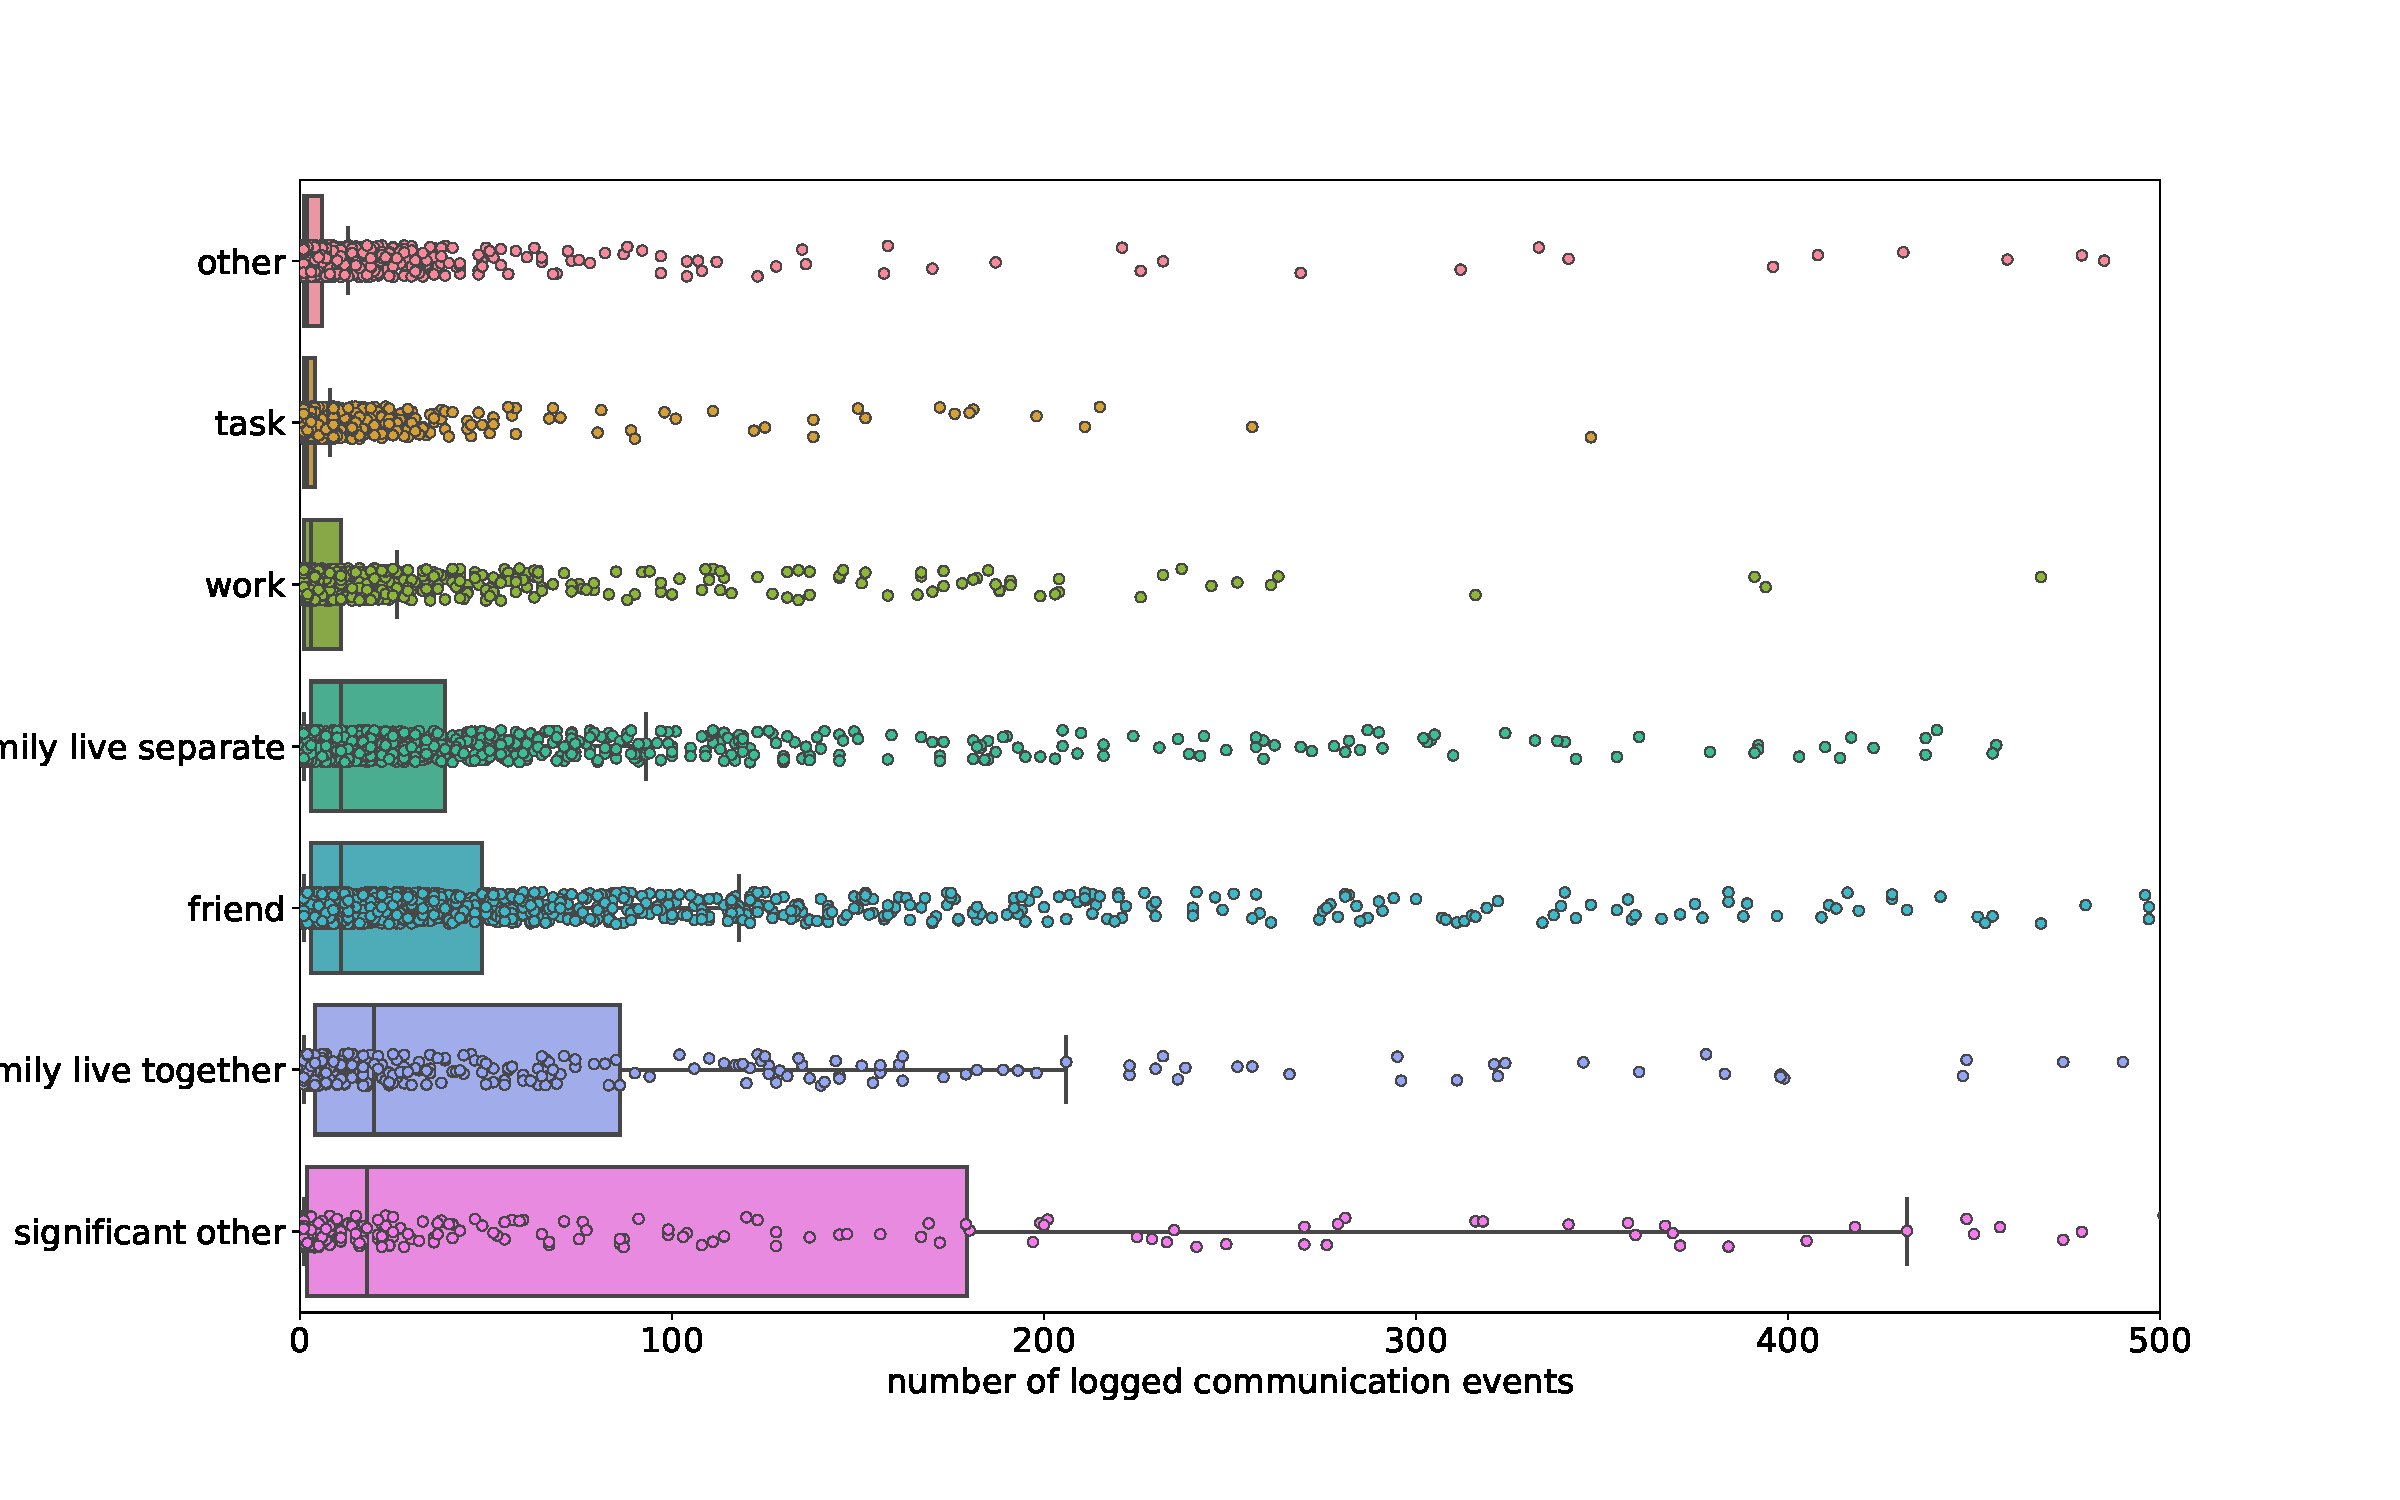
\includegraphics[width=1\textwidth]{figures/all_contact_types_comm_freq_strip.pdf}
    %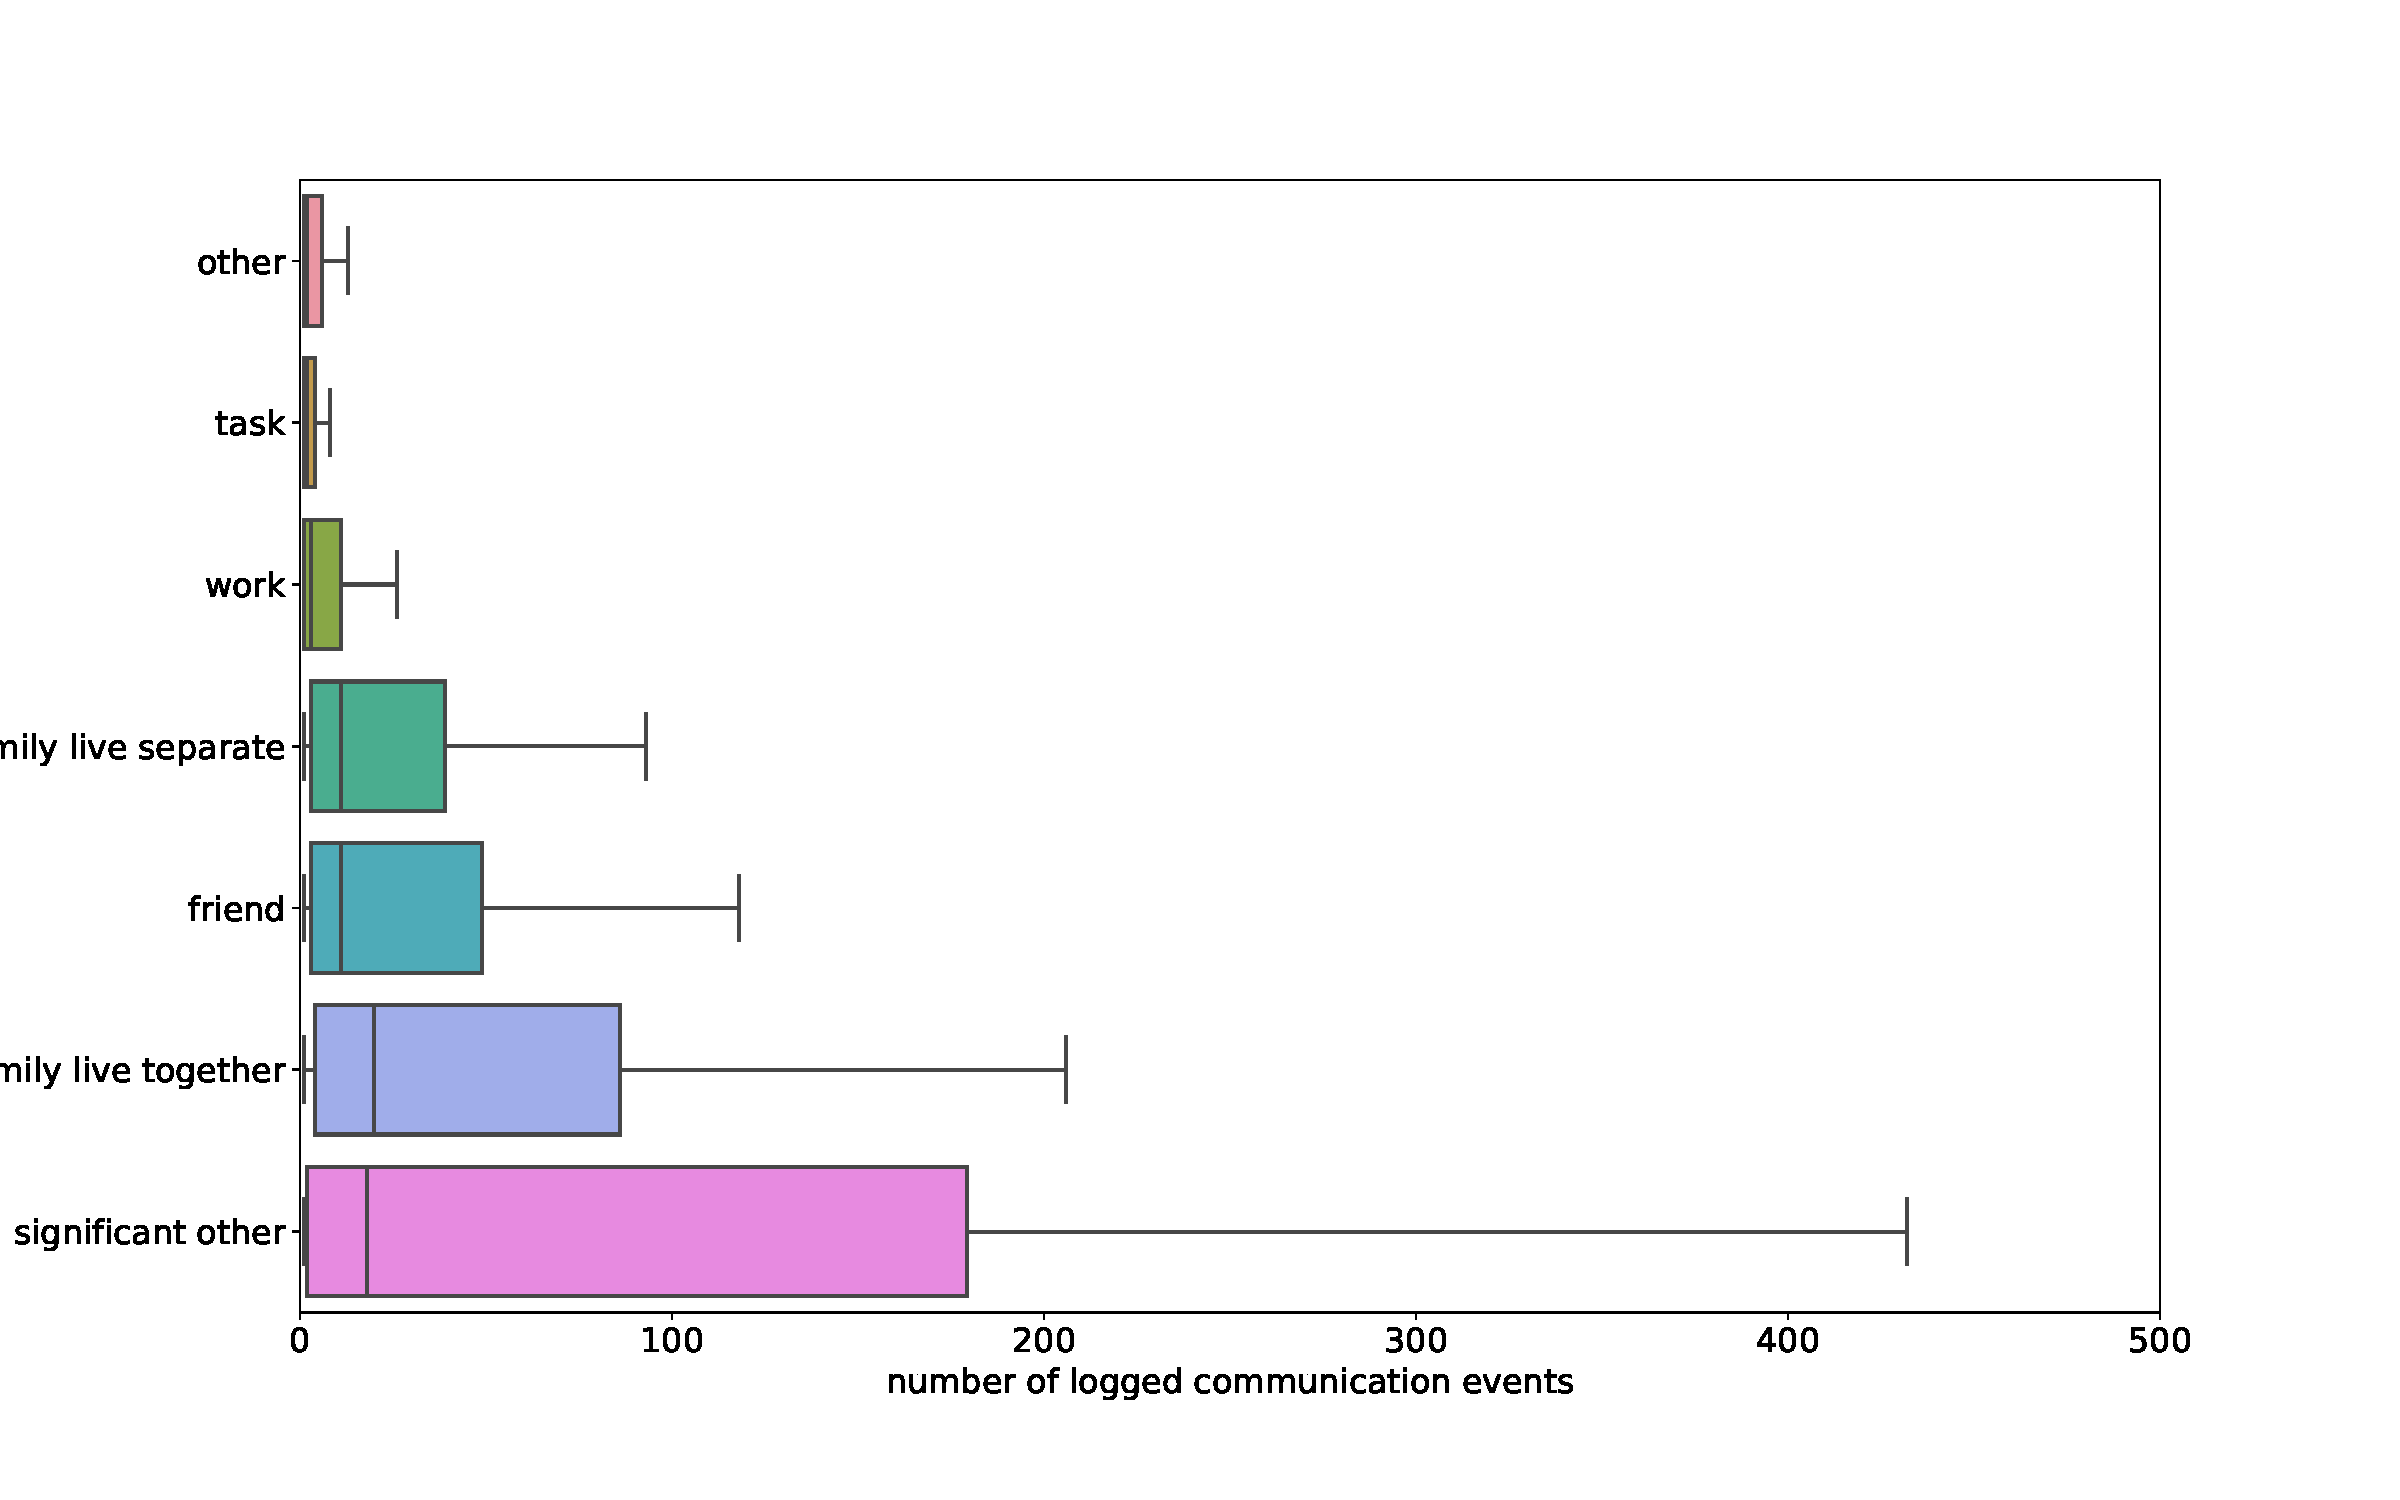
\includegraphics[width=1\textwidth]{figures/all_contact_types_comm_freq.pdf}
    \caption{\textbf{The relationship between contact type and communication frequency across all contacts}. Points overlaid on the box plots are individual contacts in our data. When considering all participants' contacts, we see that the vast majority of ``other'' and ``task'' contacts have few logged communication events, illustrating the need for a communication frequency cutoff to model the contacts that truly provide social support for their corresponding participant.}
    \label{fig:comm_frequency}
\end{figure}



\subsection{Feature extraction}
\label{subsec:feature_extract}
For our prediction tasks, we consider a number of feature blocks: communication, demographics, and semantic location.

\subsubsection*{Communication features}

We derive 147 communication features based on previous work by~\cite{min2013mining}, replicating all of their features except for those relating to SMS length. These features fall into four broad categories as defined in~\cite{wiese2015you} and others:

% TODO elaborate on the broad categories
\begin{itemize}
    \itemsep0em
    \item \textit{intensity and regularity}: features that consider the volume and regularity of communication, such as mean or median weekly calls or number of study days with a logged communication.
    \item \textit{temporal tendency}: features that capture the time of day or day of week when communication events typically occur.
    \item \textit{channel selection and avoidance}: features that capture any asymmetry in communication (incoming vs. outgoing) or preference for calls vs. SMS.
    \item \textit{maintenance cost}: features that consider the amount of effort in maintaining communication relationships.
\end{itemize}

% remove hyperlinks for paper submission
A full description of these features as well as summary statistics can be found at our project's Github page (Figure~\ref{fig:comm_features}).

%\href{https://github.com/tliu526/relationship-prediction/blob/master/feature_extract/feature_extract.ipynb}{Github page}



\subsubsection*{Demographic features}

We also wish to evaluate how demographics impact communication patterns and consequently social relationship inference. Thus, we treat demographic information about each participant as separate feature blocks. This included age, gender, race, ethnicity, education, marital status, employment status, and whether the participant lived alone or with others. All of the categorical responses were encoded in a one-hot representation. Summary statistics of our participant demographics can be found in Table~\ref{tab:demo_info}.

\subsubsection*{Semantic location features}

To convert the raw GPS data into higher-level features, we use the adaptive k-means clustering methodology presented in~\cite{saeb2017mobile}. First, GPS readings were clustered with a maximum radius of 100 meters. Clusters that had durations of fewer than 10 minutes were discarded to handle transient locations, such as when a participant was stuck in traffic. Participants then answered two questions about the detected location clusters: ``what kind of place is this?" and ``why did you visit this place''? Responses were chosen from pre-defined categories, with options such as ``home'' or ``nightlife spot'' for the place type and ``entertainment'' or ``errand'' for the visit reason. A full list of the possible survey responses can be found in the Appendix. % TODO add to appendix

We then cross-reference the duration of time each participant spent at a location with their communication logs, so that an individual call or text could be labelled as sent or received from a particular location (Figure~\ref{fig:semantic_location}). These counts are normalized over all communication events for each contact, giving us relative proportions of communication events that occur at a semantic location.

% TODO update with own styling
\begin{figure*}
    \centering
    \includegraphics[width=1\textwidth]{figures/semantic_loc.png}
    \caption{\textbf{Semantic location chart over the study period for a representative participant.} We see some regularity in the participant's visits to ``home'' and ``work'' locations. }
    \label{fig:semantic_location}
\end{figure*}

\subsubsection*{Missing Data Imputation}

Due to the passive nature of how phone sensor data are collected, missing data are commonplace and needs to be appropriately handled. Furthermore, it is often the case that data are not missing at random, and the presence or absence of a feature can provide information (eg, a lack of calls to a contact between 12 am and 4 am). To this end, we not only impute missing features with the sample population median but also include a new indicator feature for whether the data are missing. This allows us to capture any potential patterns in how data are missing, which could provide additional information to the predictive models.

\subsection{Predictive modeling and procedural setup}


\subsubsection*{Cross validation methodology}

Because there is shared information between contacts sourced from the same participant, it is critical that we cross-validate over participants as opposed to over contacts to ensure that there is no data leakage. Saeb et al demonstrate that improper cross validation not only incorrectly inflates performance metrics, but also fails to measure the generalization of a model on true out-of-sample data~\cite{saeb2016voodoo}. In the context of relationship prediction, contacts that are associated with a particular participant could have similar communication tendencies based on individual variation as well as identical demographics, which could bias our model's estimation by potentially learning to identify individual participants as opposed to actually learning the characteristics of relationship classes. To this end, we train our models using \textit{grouped} $K$-fold cross validation, where all the contacts $c \in C_i$ associated with a participant $i$ are included in a single fold and the $K$ folds are defined in terms of groups of participants $P_k$ (Equation~\ref{eq:group_cv}). This cross-validation methodology ensures that our models do not over-fit the training data, producing meaningful performance results.

% TODO should this be captioned?
\begin{equation}
    \label{eq:group_cv}
    % TODO which is more readable?
    % \mathcal{L} = \sum^K_{k=1} \Big [ \sum_{i \in P_k} \frac{1}{|C_i|} \sum_{c \in C_i} \mathbf{1}\{\hat{y}_c \ne y_c\}\Big ]
    \mathcal{L} = \sum^K_{k=1} \Big [ \sum_{i \in P_k} \frac{\sum_{c \in C_i} \mathbf{1}\{\hat{y}_c \ne y_c\}}{|C_i|} \Big ]
\end{equation}

\subsubsection*{Automated machine learning}

% TODO CCC
We utilize \textit{auto-sklearn}~\cite{feurer2015efficient} for our feature selection, model selection, and hyperparameter tuning process. Model building occurs in three stages. First, a meta-learning step selects promising initializations of hyperparameters based on the given data's similarity to existing data. Next, specific algorithms and hyperparameter settings are tuned through Bayesian optimization~\cite{brochu2010tutorial}. Finally, the best models found through this optimization process are used to automatically construct an ensemble model, which is the final model output. Automatic selection of model parameters and ensembling not only tends to give slightly higher performance than manually engineering them, it also prevents any user bias from being introduced into the resulting model, such as a preference for one algorithm over another or prior knowledge about the dataset that can be exploited. Auto-sklearn is feature and algorithm agnostic, allowing us to essentially treat the model building process as a hands-off task.

% TODO add back repository information after review process
% Details on our exact auto-sklearn settings can be found in our Github repository.

\subsubsection*{Feature importance analysis using SHAP}

We not only want a model with good performance --- we would also like to interpret the relative importance of features when it makes predictions. However, because auto-sklearn builds ensembles of various machine learning models for its final output, feature weights are not directly accessible. Our solution is to use \textit{SHAP}, which combines numerous additive feature attribution techniques to produce a single ``explanation model''~\cite{lundberg2017unified}. The intuition behind these methods is that they map the original features of a local data point $x$ to a simplified space where the mapped inputs contribute additively to a linear explanation model. These features can then be easily assigned importance based on their contributions to the explanation model, which also describes the actual classifier output for $x$. By using SHAP, we are able to give more intuitive analyses of our models' performance despite their complexity.

\section{Results: Relationship Prediction Analysis}
\label{sec:rel_pred_results}

To make progress at relationship prediction we need to choose the features and an evaluation procedure. We use the following feature sets: 
\begin{itemize}
    \itemsep0em
    \item age and gender
    \item communication features
    \item communication + age/gender features 
    \item communication + demographics + semantic location features
\end{itemize}
We hold out 25\% of the participants as an out-of-sample test set, and use accuracy, weighted F1 and macro F1 to evaluate final model performance. Random forests trained using the auto-sklearn framework serve as a baseline comparison to the auto-sklearn ensemble methods. These choices enable us to quantify relationship prediction as a function of the type of the feature set.

\subsection{Four-class Relationship Prediction Performance}
% TODO correct term for peer family members?
% TODO we'll likely need to justify more why we chose to collapse classes
For a meaningful comparison across relationship roles we must have classes that are sufficiently distinct. We first trained our models for relationship prediction utilizing all six relationship categories: ``family live together,'' ``family live separate,'' ``friend,'' ``work,'' and ``task.'' In these initial runs, we found that ``family live separate'' and ``friend'' contacts are often confused. We hypothesize that instead of predicting the social role, our models were detecting the structure of the relationship in whether the participant lives with the contact or not. This could have more impact on when and how participants communicate with contacts than any familial labels: communication patterns between ``peer'' family members who live separately such as siblings can bear closer resemblance to social relationships than other familial relationships. To this end, we define new labels where the  ``family live separate'' and ``friends'' labels are collapsed into a single category: ``social separate,'' and ``significant other'' and ``family live together'' labels are collapsed into a single category: ``family together.'' We note that the six-class prediction class results show similar trends in performance across the blocks of features, which can be found in Supplemental Figure~\ref{tab:top5_6class_metrics} and Supplemental Table~\ref{tab:top5_6class_metrics}. For the rest of our paper we thus focus on the four-class prediction task for model evaluation. 


\begin{table}[h!]
    \centering
        \begin{tabular}{llcccc}
        \toprule
                     model &    features &  accuracy &  macro f1 &  weighted f1 \\
        \midrule
         majority baseline &         N/A &    0.5714  &    0.1818 &       0.4156 \\
         \midrule
            random forest & age/gender & 0.5714 &    0.1818 &       0.4156 \\
             random forest &    comm &    0.6667 &    0.4795 &       0.6254 \\
             random forest &  comm + age/gender &    0.6667 &    0.4750 &       0.6225 \\
    %         Random forest &        demo &    0.6667 &    0.4598 &       0.6213 \\
             random forest & comm + demo + loc &    0.6762 &    0.4744 &       0.6326 \\
        \midrule
                    auto-sklearn & age/gender & 0.5714 &    0.1818 &       0.4156 \\
                    auto-sklearn & comm &    0.6571 &    0.4731 &       0.6195 \\
                    auto-sklearn &  comm + age/gender &    0.6905 &    0.5488 &       0.6654 \\
    %                auto-sklearn &        demo &    \textbf{0.7095} &             \textbf{0.5344} &    \textbf{0.5598} &       0.6775 \\
                    auto-sklearn & comm + demo + loc &    \textbf{0.7095} &    \textbf{0.5519} &       \textbf{0.6806} \\
        \bottomrule
        \end{tabular}

        \caption{\textbf{Performance metrics for the four-class relationship prediction task.} We show the highest scores in bold. Auto-sklearn is used for hyperparameter selection of the ``random forest'' models, while the ``auto-sklearn'' models are ensembles of the best performing models found via auto-sklearn's optimization process. Feature blocks correspond to the four feature configurations described above, with ``comm'' as communication features, ``demo'' as all demographic features, and ``loc'' as semantic location features. }
        \label{tab:top5_4class_metrics}
\end{table}

Our goal is to measure any improvement in relationship prediction when adding demographics and location features. Indeed, we find that including these features help model performance (Table~\ref{tab:top5_4class_metrics}). First, we note that due to class imbalance across our data the trivial strategy of always guessing the majority baseline (``social separate'') in fact sets a meaningful lower bound of performance to compare against. Our best performing model, the auto-sklearn ensemble trained with all of our features, achieves an accuracy of 71\% on the held-out test set, a 14 point increase in raw accuracy over the majority baseline prediction. Improvements over baseline are larger in the F1 scores with the ensemble model producing a macro F1 of 0.55 and a weighted F1 of 0.68. Across all metric comparisons we find that adding demographics and location features considerably improves prediction performance.

% TODO paragraph on auto-sklearn comparison
%A general trend we note is that the auto-sklearn ensemble models perform slightly better than the tuned random forest models, especially when trained with more features.

%TODO how to better conclude confusion matrix discussion? Doesn't quite fit with the feature analysis motivation. 
When evaluating performance, it is important for us to also consider misclassified contacts as they can provide information on the relationship between our contact types. We find that the across all types, the most common confusion is incorrectly predicting ``social separate'' (Table~\ref{tab:top5_4class_confusion}), which is not surprising given the class imbalance we have noted. Despite this, classification performance of ``task'' and ``family together'' labels is reasonable with accuracies of about 60\%. On the other hand, ``work'' contacts are almost entirely misclassified as ``social separate'' contacts. We hypothesize that given we only consider the top five contacts of each participants, contacts nominally labelled ``work'' are in fact contacts the participant is closer to, akin to a friend. This motivates the need to consider finer-grained contact types or alternative measures of social roles as contact type labels sometimes do not capture the complete context of a social relationship.

\begin{table}[h]
    \centering
        \begin{tabular}{lcccc}
        \toprule
        {} &  pW &  pSS &  pT &  pFT \\
        \midrule
        W            &       1 &        15 &       0 &                  0 \\
        SS          &       0 &       106 &       1 &                 13 \\
        T            &       0 &         7 &      11 &                  1 \\
        FT &       0 &        23 &       1 &                 31 \\
        \bottomrule
        \end{tabular}
        \caption{\textbf{Test set confusion matrix for the ``auto-sklearn'' ensemble model with all features.} Contact types are abbreviated work (W), social separate (SS), task (T), and family together (FT), and  columns, marked by ``p,'' are predictions. We see reasonable performance on the majority of contact types given the class imbalance present within our data, though most ``work'' contacts are misclassified.}
        \label{tab:top5_4class_confusion}
\end{table}

Breaking our model features into four separate configurations also allow us to examine relative changes in performance when introducing particular features. Across the ``auto-sklearn'' feature blocks (Table~\ref{tab:top5_4class_metrics}), we see the largest increase in performance when adding age and gender to our model with a 3.4\% bump in accuracy and 4.5 point increase in weighted F1, while including other demographics and location features on top of age and gender provide much smaller performance improvements. This increase when introducing age and gender features is particularly interesting when we consider the fact that age and gender features alone do not appear to have any predictive value: as shown in Table~\ref{tab:top5_4class_metrics}, models trained using only those features do no better than simply guessing the majority class. This is an indication that there is a potential interaction effect between age/gender and the other features, particularly communication features, that leads to the improvement in performance.

% \begin{table}[]
%     \centering
%         \begin{tabular}{llcccc}
%         \toprule
%                      model &    features &  accuracy &  balanced accuracy &  macro f1 &  weighted f1 \\
%         \midrule
%          majority baseline &         N/A &    0.5714 &             0.2500 &    0.1818 &       0.4156 \\
%          \midrule
%              Random forest &    comm &    0.6667 &             0.4590 &    0.4795 &       0.6254 \\
%              Random forest &  comm + age/gender &    0.6667 &             0.4566 &    0.4750 &       0.6225 \\
%     %         Random forest &        demo &    0.6667 &             0.4369 &    0.4598 &       0.6213 \\
%              Random forest & comm + demo + loc &    0.6762 &             0.4546 &    0.4744 &       0.6326 \\
%         \midrule
%                     auto-sklearn & age/gender & 0.5714 &             0.2500 &    0.1818 &       0.4156 \\
%                     auto-sklearn & comm &    0.6571 &             0.4598 &    0.4731 &       0.6195 \\
%                     auto-sklearn &  comm + age/gender &    0.6905 &             \textbf{0.5310} &    0.5488 &       0.6654 \\
%     %                auto-sklearn &        demo &    \textbf{0.7095} &             \textbf{0.5344} &    \textbf{0.5598} &       0.6775 \\
%                     auto-sklearn & comm + demo + loc &    \textbf{0.7095} &             0.5221 &    \textbf{0.5519} &       \textbf{0.6806} \\
%         \bottomrule
%         \end{tabular}

%         \caption{Performance metrics for the 4 class relationship prediction task with highest scores in bold. Feature blocks correspond to the configurations described above, with ``comm'' as communication features, ``demo'' as all demographic features, and ``loc'' as semantic location features.}
%         \label{tab:top5_4class_metrics}
% \end{table}


\subsection{Feature Importance}

Now that we have seen that the addition of demographic and semantic location features improve model performance, we wish to explore feature interactions with the various contact types as well as gain insight on their fine-grained effects on relationship prediction performance. To accomplish this, we use the SHAP framework to examine predictive feature importance across both individual features and our pre-defined feature blocks. Our analysis provides a degree of explanation as to why our models made their predictions and also sheds some light on specific communication patterns that characterize particular contact types.

%\subsubsection*{SHAP feature analysis}

We know from our feature block setup that communication features are critical for good performance (Table~\ref{tab:top5_4class_metrics}), but we would like to gain some insight on features are actually contributing to model predictions for particular contact types. By examining the average SHAP magnitude, we see that that all but two of the top fifteen most important features are derived from communication patterns (Figure~\ref{fig:top5_ag_shap}), which is expected given the modest increases in performance when comparing the models trained with only communication features to our models with additional demographic and location features. Out of the four categories of communication features we construct (Section~\ref{subsec:feature_extract}), \textit{intensity and regularity} (total communication days, call duration, communication regularity) and \textit{temporal tendency} (communications made between 8pm and 12am, 12am and 4 am, and on Sunday) are particularly prominent. The most important individual feature, total number of days of communication, is a strong signal for the ``family together'' and ``social separate, '' which is an intuitive relationship as this feature encapsulates both the regularity and volume of communication. Through SHAP analysis of our features, we are able to see that the timing as well as the volume of communication are the most important factors in determining the nature of relationships participants have with close contacts.

We would ideally also want to observe the relative contributions features make to particular relationship classes, even the ones that are sparsely represented such as ``work'' and ``task''. Our SHAP analysis in fact enables us to do so. The features that contribute the most to a ``work'' classification are texts on Mondays and calls between 8 am and 12 pm (Figure~\ref{fig:top5_ag_shap}). Intuitively, communications during these time periods would be indicative of work-related interactions, demonstrating that communication patterns we would expect to be important for the ``work'' contact type in fact are the most useful for differentiating it in the data. Regarding ``task'' contact types, we see that the total number of communications as well as the missed to incoming call ratio are particularly important for the class. Again, these features appeal to our intuition: ``task'' contacts should communicate in much lower volume with a participant than the other contact types, and the proportion of missed calls from a ``task'' contact should be much higher perhaps due to the relative unimportance of the communications or a lack of desire for participants to engage with these contacts. Thus, despite the presence of class imbalance in our underlying data, this method of feature analysis still allows us to draw inferences on which features contribute to the rarer classes.

Additionally, the SHAP feature importances highlight the contributions of certain semantic location features to our model outputs. We see that calls taken at locations where the the visit reason was ``errand'' and calls taken at shops are important (Figure ~\ref{fig:top5_ag_shap}). These two features make the largest contributions to the ``family together'' class output, a sensible result as communications while running errands or shopping (eg for groceries in a common household) will likely be made to contacts that live with the participant. This analysis demonstrates the value in including semantic location features as it can further contextualize communication events for particular contact types.

% Notably absent in the top SHAP values however are demographic features, particularly age and gender. We hypothesize that there is an interaction effect...

\begin{figure}[h]
    \centering
    \includegraphics[width=0.8\textwidth]{figures/top5_all_shap.pdf}
    \caption{\textbf{Top 15 features of the best performing auto-sklearn model ordered by average SHAP value magnitude.} We see that features related to communication volume, regularity, and temporality are important. Additionally, we are able to visualize the relative contributions of each feature to a particular contact type output. }
    \label{fig:top5_ag_shap}    
\end{figure}



\subsection{Age Interaction with Communication Patterns}

\begin{table}[h]
    \centering
    \begin{tabular}{lrr}
    \toprule
    communication features &   corr &     p \\
    \midrule
    call tendency                             &  0.181 & <0.001 \\
    12am - 4am communication                  & -0.146 & <0.001 \\
    12am - 4am SMS                            & -0.145 & <0.001 \\
    8pm - 12am SMS                            & -0.141 & <0.001 \\
    texting regularity                        & -0.139 & <0.001 \\
    Sunday SMS                                & -0.132 & <0.001 \\
    total \# texting days                     & -0.131 & <0.001 \\
    communication within last 2 weeks         &  0.129 & 0.001 \\
    Sunday communication                      & -0.128 & 0.001 \\
    Max incoming SMS frequency                & -0.118 & 0.002 \\
    8pm - 12am communication                  & -0.116 & 0.002 \\
    standard deviation incoming SMS frequency & -0.111 & 0.004 \\
    call duration within last 2 weeks         &  0.110 & 0.005 \\
    mean incoming SMS frequency               & -0.110 & 0.005 \\
    median incoming SMS frequency             & -0.108 & 0.006 \\
    median outgoing SMS frequency             & -0.107 & 0.006 \\
    SMS frequency within last 2 weeks         & -0.103 & 0.009 \\
    Max outgoing SMS frequency                & -0.103 & 0.009 \\
    \bottomrule
    \end{tabular}
    \caption{\textbf{Participant age correlations with communication features.} We show significant features with a false discovery rate of <0.01~\cite{benjamini1995fdr}, sorted by correlation magnitude. The most notable trends are that there is a shifting preference from texts to calls and that late night communications become less frequent as age increases.}
    \label{tab:age_comm_corr}
\end{table}



\section{Results: Subgroup Generalization Task}
\label{sec:subgroup_results}

 Many studies in the personal sensing and relationship prediction literature utilize student samples which are skewed towards younger age demographics, raising questions about their generalizability. We have shown in the previous section that participants of different ages have distinct communication patterns, which will likely impact relationship prediction model performance when applied to out-of-sample populations. To quantify this effect, we conduct a prediction task where we split our data into quartiles by age, train models within each quartile, and evaluate performance on the other quartiles. In order to have consistent comparisons across our relationship prediction tasks, we mirror the best-performing setup on our original relationship prediction tasks presented in Section~\ref{sec:rel_pred_results} by utilizing auto-sklearn with all of our derived features (communication, demographics, semantic location) and the same within-participant cross-validation procedure to train models on our four quartile subgroups. This across-group prediction task allows us to measure how age homogeneity may affect generalization.
 
 %To quantify the effect of homogeneous training samples on out-of-sample model performance, we split our data into quartiles by age, train models within each quartile, and evaluate model performance on the other quartiles. Conducting this across-group prediction task allows us to measure how age homogeneity may affect generalization. 

\subsection{Subgroup Data Description and Setup}

% TODO drop in correlation analysis across groups?
We need to understand the composition of each of our subgroup populations in order to ensure our prediction task properly evaluates model generalizbility. We initially considered a subdivision where groups were constructed based on whether participants were students, however we lacked the requisite sample size for a meaningful comparison across these groups. We also considered specific age cut-offs (eg participants under the age of 25), but decided that quartile boundaries set according to our data distribution would be the cleanest experimental setup for defining subgroups. The first quartile spans 18 to 31 year-olds and contains 52 participants, the second quartile spans 32 to 37 year-olds and contains 43 participants, the third quartile spans 38 to 46 year-olds, and the fourth quartile spans 47 to 66 year-olds (Figure~\ref{fig:subpop_age_hist}). We note that the number of participants and thus contacts are roughly the same in each quartile, so none of the models will have an undue advantage in training set size. Overall, we find that the quartile subgroup splits provide a clean methodology for evaluating relative model performance across different populations.

\begin{figure}
    \centering
    \includegraphics[width=0.75\textwidth]{figures/q_age_hist.png}
    \caption{\textbf{Histogram of participant ages with quartile cutoffs.} As defined by the distribution of participant ages in our sample, the cutoffs are defined at age 31 (Q1 to Q2), 37 (Q2 to Q3), and 46 (Q3 to Q4). }
    \label{fig:subpop_age_hist}    
\end{figure}

\begin{table}[]
    \centering
        \begin{tabular}{lrrrr}
        \toprule
        {} &  family together &  social separate &   task &  work \\
        \midrule
        Q1 &           20.38\% &           67.31\% &  5.00\% & 7.31\% \\
        Q2 &           25.58\% &           56.74\% & 10.70\% & 6.98\% \\
        Q3 &           24.71\% &           58.43\% &  8.63\% & 8.24\% \\
        Q4 &           21.86\% &           56.74\% & 12.09\% & 9.30\% \\
        \bottomrule
        \end{tabular}
    \caption{\textbf{Percentage of relationship labels within each age quartile.} Distributions are approximately equal across Q2, Q3, and Q4, while Q1 has roughly 10\% more ``social separate'' contacts.}
    \label{tab:subpop_contact_types}
\end{table}

Understanding the distribution of contact types within each group is also important when examining subgroup model performance. We see that though the proportion of each contact type is approximately the same across Q2, Q3, and Q4, Q1 has a larger amount of ``social separate'' labels when compared to the other quartiles (Table~\ref{tab:subpop_contact_types}). To address these relative differences between the proportion of contact types per quartile, labels are resampled so that all classes are equally represented in each cross-validation fold of the training procedure. Additionally, we choose to use macro F1 as our target metric to account for the class imbalance across our quartile samples; by evaluating our models using macro F1, trained models cannot artificially achieve higher out-of-sample performance simply by predicting the majority class. We note that the weighted F1 metrics (Supplemental Table~\ref{tab:subpop_perf_weight}) produces qualitatively the same trends as our subsequent performance analysis that focus on macro F1. These resampling and performance metric choices make the relative performances of each subgroup model more comparable.

% Here, we see that there are differences this distribution per quartile that could potentially impact relative model performance. 

Analogous to our question regarding the limits of model generalizability when trained on homogeneous samples, we also hypothesize that models trained on \textit{heterogeneous} data are able to generalize better across a wider test set population. To this end, we include model runs where we sample twelve participants from each quartile (48 participants total) to produce a heterogeneous training set and evaluate out-of-sample performance on the rest of the data --- this ``allQ'' model result is calculated as the mean performance over ten such samples drawn. The ``allQ'' model configuration allows us to evaluate the impact of having more varied training data on out-of-sample model performance.

\subsection{Subgroup Model Performance}

% TODO would be cool to plot the cumulative feature importance of SMS vs call features as function of the quartiles -> hopefully see a decrease in importance of SMS features as we go to higher quartiles

% Macro F1 results support our story the best
% "We use macro F1 because it has high dynamic range -> class imbalance doesn't help it"

% Within sample performance, as indicated by italics, are obtained by 5-fold cross validation and provide a benchmark for the best performance that can be achieved for that particular subgroup.

Though we naturally expect lower out-of-sample performance for our subgroup-trained models, we are interested in trends in relative performance across our models that can give insight for the generalizability of particular age quartiles. Indeed, we see that the model trained on the Q1 subgroup generalizes particularly poorly across the other subgroups, producing the worst performance out of all other models for its out-of-sample test subgroups (Table~\ref{tab:subpop_perf_macro}). Additionally, the Q2, Q3, and Q4-trained models produce their respective lowest test performance values on the Q1 subgroup. This could be due to the differences in class label distribution of the Q1 subgroup in comparison to the others (Table~\ref{tab:subpop_contact_types}), though our resampling of the training data would mitigate this effect. This could also be due to differences in the distribution of features in the Q1: for example, we have already seen that younger people have higher texting regularity than older people, which could result in the model trained on only Q1 data to over-emphasize texting features, leading to poor out-of-sample performance when those features are not as indicative of relationship labels in the older subgroups. Regardless of the exact source of this discrepancy in performance, what we have seen is that the youngest quartile in our sample is fundamentally different in both feature and relationship label composition than the rest of our sample. 

Furthermore, this experiment also illustrates the benefits of having a heterogeneous training sample. Our ``allQ''-trained models (last row of Table~\ref{tab:subpop_perf_macro}) produce the best average test performance across all four quartiles, and in all subgroups except for Q4. Performance of the overall model is within a standard deviation of the in-sample performance. This result is not entirely surprising, as when given a training set with more variance, models should generalize better to out-of-sample data. Still, the superior performance of the ``allQ''-trained models when compared to the others that are trained on more homogeneous data emphasize the standard lessons of machine learning, namely that ML techniques are good at interpolation not extrapolation of data.

% TODO move to discussion
% and that 

\begin{table}[h]
    \centering
    \begin{tabular}{lllll}
    \toprule
    Model &  q1 macro f1 &  q2 macro f1 &  q3 macro f1 &  q4 macro f1 \\
    \midrule
    majority &        0.205 &        0.174 &        0.183 &        0.184 \\
    q1-trained model       &        \textit{0.418} &        0.315 &        0.386 &        0.349 \\
    q2-trained model       &        0.353 &        \textit{0.479} &        0.426 &        0.456 \\
    q3-trained model       &        0.312 &        0.450 &        \textit{0.483} &        0.443 \\
    q4-trained model       &        0.321 &        0.455 &        0.397 &        \textit{0.587} \\
    allq-trained model     &        0.388 $\pm$ 0.038 &        0.468 $\pm$ 0.021 &        0.425 $\pm$ 0.022 &        0.487 $\pm$ 0.041 \\
    \bottomrule
    \end{tabular}
    \caption{\textbf{Performance of models trained on different sample subgroups, optimizing for macro F1.} Each row corresponds to a model trained on the indicated age quartile. Within sample results are obtained by 5-fold cross validation, indicated by italics.
    All-quartile models are trained on an equal number of participants sampled from each quartile, with the sampling procedure conducted ten times to produce the final average performance and standard deviations indicated.}
    \label{tab:subpop_perf_macro}
\end{table}

% \begin{itemize}
% \item Subpopulation prediction: we need to train on the right subjects $\rightarrow$ Really get towards the standard lessons of ML, interpolation etc (Tables ~\ref{tab:subpop_perf_weight},~\ref{tab:subpop_perf_macro})
%     \begin{itemize}
%         \item hypothesis: people of different ages have fundamentally different communication patterns --- ``students aren't people''
%         \item subdivide our sample population into quartiles
%         \item train models on resampled data within each quartile to account for class imbalance
%         \item models trained on youngest subpopulation generalized the worst
%         \item point to macro F1 scores for how a more heterogeneous mix of samples improves performance
%     \end{itemize}
% \end{itemize}



% \begin{table}[H]
%     \begin{tabular}{lllll}
%     \toprule
%     Model &  q1 micro f1 &  q2 micro f1 &  q3 micro f1 &  q4 micro f1 \\
%     \midrule
%     majority &        0.655 &        0.561 &        0.600 &        0.574 \\
%     q1-trained model       &        \textit{0.700} &        0.600 &        0.600 &        0.586 \\
%     q2-trained model       &        0.700 &        \textit{0.646} &        0.631 &        0.605 \\
%     q3-trained model       &        0.692 &        0.651 &        \textit{0.643} &        0.651 \\
%     q4-trained model       &        0.665 &        0.628 &        0.671 &        \textit{0.656} \\
%     allq-trained model     &        0.683 $\pm$ 0.026 &        0.628 $\pm$ 0.019 &        0.600 $\pm$ 0.026 &        0.628 $\pm$ 0.041 \\
%     \bottomrule
%     \end{tabular}
%     \caption{Performance of models trained on different sample subgroups, optimizing for micro F1. Each row corresponds to a model trained on the indicated age quartile. Within sample results were obtained by 5-fold cross validation and are indicated by italics.
%     All-quartile models are trained on an equal number of participants sampled from each quartile, with the sampling procedure conducted ten times to produce the final average performance and standard deviations indicated.}
%     \label{tab:subpop_perf_micro}
% \end{table}



\section{Discussion}
\label{sec:discussion}

\begin{itemize}
    \item How we filled the gap
    \begin{itemize}
        \item Analysis of interaction between demographics/semantic location with communication, yielding improvement in model performance
        \item Demonstration of the limits of generalizability in personal sensing models, and an exploration of why the differences in performance across age groups occur
        \item Note the difference in performance across papers $\to$ emphasizes the point of generalization
    \end{itemize}
    \item Our limitations
    \begin{itemize}
        \item Though large for the community, we still have relatively small $n$ 
        \item We also have a biased sample of our own, skewed towards females
        \item Our choice of prediction task may be limited, only considering top 5 vs all contacts
    \end{itemize}
    \item Future work
    \begin{itemize}
        \item Exploration of population heterogeneity across mood disorders
        \item Incorporation of data provenance to predictive models
    \end{itemize}
    \item Wider impact
    \begin{itemize}
        \item Results highlight the promise of passive sensing: additional feature modalities increase performance and reveal insights into individual communication patterns
        \item Also illustrate how many predictive modeling studies must be taken with a grain of salt: generalization and overfitting are great concerns the community must be mindful about
        \item our results should motivate future studies to strongly consider collecting heterogeneous data
        \item homogeneity is everywhere: even if one is only interested in modeling students, ensuring that the samples comes from a varied sample (eg not all psychology or computer science majors) can improve out-of-sample model performance
    \end{itemize}
\end{itemize}

% How we filled the gap
% TODO discuss differences in performances between our model and others
% they have a more homogeneous sample, fewer class labels, and "easier" contacts (not top five)
We have explored the impact of utilizing demographic and semantic location information in addition to typical communication features on relationship prediction model performance. Observing the interaction between age demographics and communication patterns, we also have conducted an age subgroup model generalization experiment where we highlight both the limits of generalizability when training models on homogeneous samples as well as the benefits of training on heterogeneous ones. Our use of automatic machine techniques throughout these tasks limit manual intervention in the model building and prediction process, a practice that we believe will encourage a more standardized methodology for tackling machine learning problems. 

% significance of the inclusion of demographics and location features

% significance of our subgroup prediction task
% - young populations generalize poorly
Within our data, training on the youngest population produces particularly poor results, highlighting the need to consider a more varied sample when training and evaluating models especially given the large proportion of studies that rely on younger (eg student) populations in the personal sensing space. 
% - heterogeneous training data produce the best results
Furthermore, the ``allQ'' models that produce superior performance when training on more varied samples indicate that it would behoove studies that aim to evaluate their predictive model's effectiveness ``in the wild'' to collect heterogeneous data to train and test on.

% dedicated thought to the performance of auto-sklearn
Though auto-sklearn is clearly not a silver bullet to all machine learning problems, it does provide a reasonable benchmark of other models; significant performance gains above automatic methods likely exploit patterns in the data, which in the relatively small sample size regime of personal sensing could limit the generalizability of particular techniques.

% Our limitations
Our study has some limitations that we wish to highlight. Though our dataset is larger than what is typical within the community, our sample size is likely still inefficient to truly demonstrate applicability and robustness of models to a wider population. %TODO power calculation citation

% Future Work
We also see an opportunity in improving model performance where features are derived from disparate data sources, which is common in the personal sensing field. By placing all sensor modalities into a single feature table, we are losing information about data provenance: semantic locations are fundamentally different than communication frequency and should be treated and regularized accordingly, yet they are analyzed in a homogeneous block. Even subcategories such as our \textit{maintenance cost} and \textit{temporal tendency} communication features carry different semantic meanings which could be useful for model creation. Future work could see applications of feature blocking techniques such as group lasso to personal sensing tasks, given the heterogeneous feature modalities of passive sensing.

% Wider Impact
Though personal sensing models have shown promise in understanding interpersonal relationships, the robustness of such models need to be validated for wider populations.

\pagebreak
\appendix

\renewcommand\thefigure{\thesection.\arabic{table}}    
\setcounter{table}{0}

\renewcommand\thefigure{\thesection.\arabic{figure}}    
\setcounter{figure}{0}

\section{Supplemental Figures and Tables}

\begin{table}[h]
    \centering
    \begin{tabular}{llrrrr}
        \toprule
        model & features & accuracy &  balanced accuracy &  macro f1 &  weighted f1 \\
        \midrule
        majority baseline & N/A &   0.3381 &             0.1667 &    0.0842 &       0.1709 \\
        \midrule
         Random forest &  comm &  0.4000 &             0.2994 &    0.2899 &       0.3559 \\
         Random forest & comm + age/gender & 0.4476 &             0.3543 &    0.3627 &       0.4123 \\
%         Random forest & comm + demo &    0.4476 &             0.3330 &    0.3291 &       0.3905 \\
         Random forest & comm + demo + loc  & 0.4333 &             0.3733 &    0.3577 &       0.4106 \\
        \hline
        auto-sklearn  & comm & 0.4524 &             0.3617 &    0.3534 &       0.4113 \\
        auto-sklearn & comm + age/gender &  0.4619 &             0.4150 &    \textbf{0.4294} &       \textbf{0.4523} \\
%        auto-sklearn & comm + demo &  0.4571 &             0.3818 &    0.3926 &       0.4344 \\
        auto-sklearn & comm + demo + loc & \textbf{0.4619} &  \textbf{0.4178} &    0.4261 &       0.4517 \\
        \bottomrule
    \end{tabular}
    \caption{Performance metrics for the 6 class relationship prediction task with highest scores in bold. Feature blocks correspond to the configurations described above, with ``comm'' as communication features, ``demo'' as all demographic features, and ``loc'' as semantic location features.}
    \label{tab:top5_6class_metrics}
\end{table}

\begin{table}[h]
    \centering
    \begin{tabular}{|lrrrrrr|}
        \hline
        {} &  pW &  pF &  pT &  pFLS &  pFLT &  pSO \\
        \hline
        W   &    2 &    7 &    0 &      6 &      0 &     1 \\
        F   &    3 &   42 &    1 &     18 &      2 &     5 \\
        T   &    1 &    3 &   14 &      1 &      0 &     0 \\
        FLS &    0 &   21 &    0 &     20 &      4 &     4 \\
        FLT &    0 &    3 &    1 &      7 &      4 &     5 \\
        SO  &    0 &   10 &    1 &      7 &      2 &    15 \\
        \hline
        \end{tabular}
        \caption{Top 5 test set confusion matrix using auto-sklearn for work (W), friend (F), task (T), family live separate (FLS), family live together (FLT), and significant other (SO) classes. Columns, marked by ``p,'' are predictions.}
        \label{tab:top5_6class_confusion}
\end{table}

\begin{table}[h]
    \centering
    \begin{tabular}{lrrrr}
    \toprule
    Model &  q1 weighted f1 &  q2 weighted f1 &  q3 weighted f1 &  q4 weighted f1 \\
    \midrule
    majority               &           0.550 &           0.411 &           0.395 &           0.359 \\
    q1-trained model       &           \textit{0.640}   &           0.507 &           0.569 &           0.519 \\
    q2-trained model       &           0.642 &           \textit{0.635}   &           0.567 &           0.585 \\
    q3-trained model       &           0.658 &           0.648 &           \textit{0.634}   &           0.623 \\
    q4-trained model       &           0.633 &           0.597 &           0.610 &           \textit{0.617}   \\
    allq-trained model     &           0.643 $\pm 0.014$ &           0.610 $\pm 0.042$ &           0.574 $\pm 0.017$ &           0.585 $\pm 0.034$ \\
    \bottomrule
    \end{tabular}
    \caption{Performance of models trained on different sample subgroups, optimized for weighted F1. Each row corresponds to a model trained on the indicated age quartile. Within sample results were obtained by 5-fold cross validation and are indicated by italics.  All-quartile models are trained on an equal number of participants sampled from each quartile, with the sampling procedure conducted ten times to produce the final average performances.}
    \label{tab:subpop_perf_weight}
\end{table}[h]

\section{Additional feature information}

\begin{figure*}
    \centering
    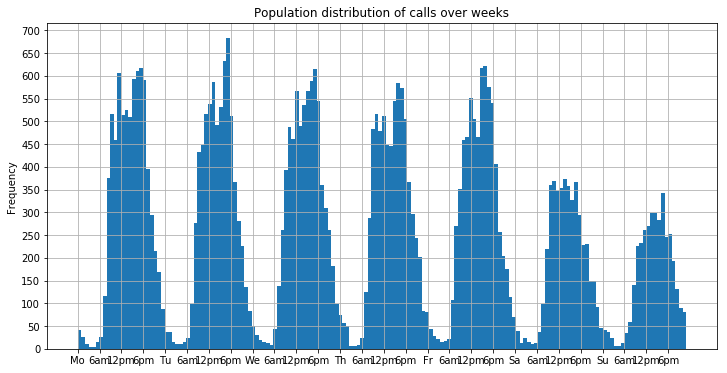
\includegraphics[width=0.8\textwidth]{figures/call_trend.png}
    \caption{Communication call patterns over days of the week. We see that there is an asymmetry between incoming/outgoing calls that is not present in SMS events.}
    \label{fig:comm_patterns}
\end{figure*}

\begin{figure*}
    \centering
    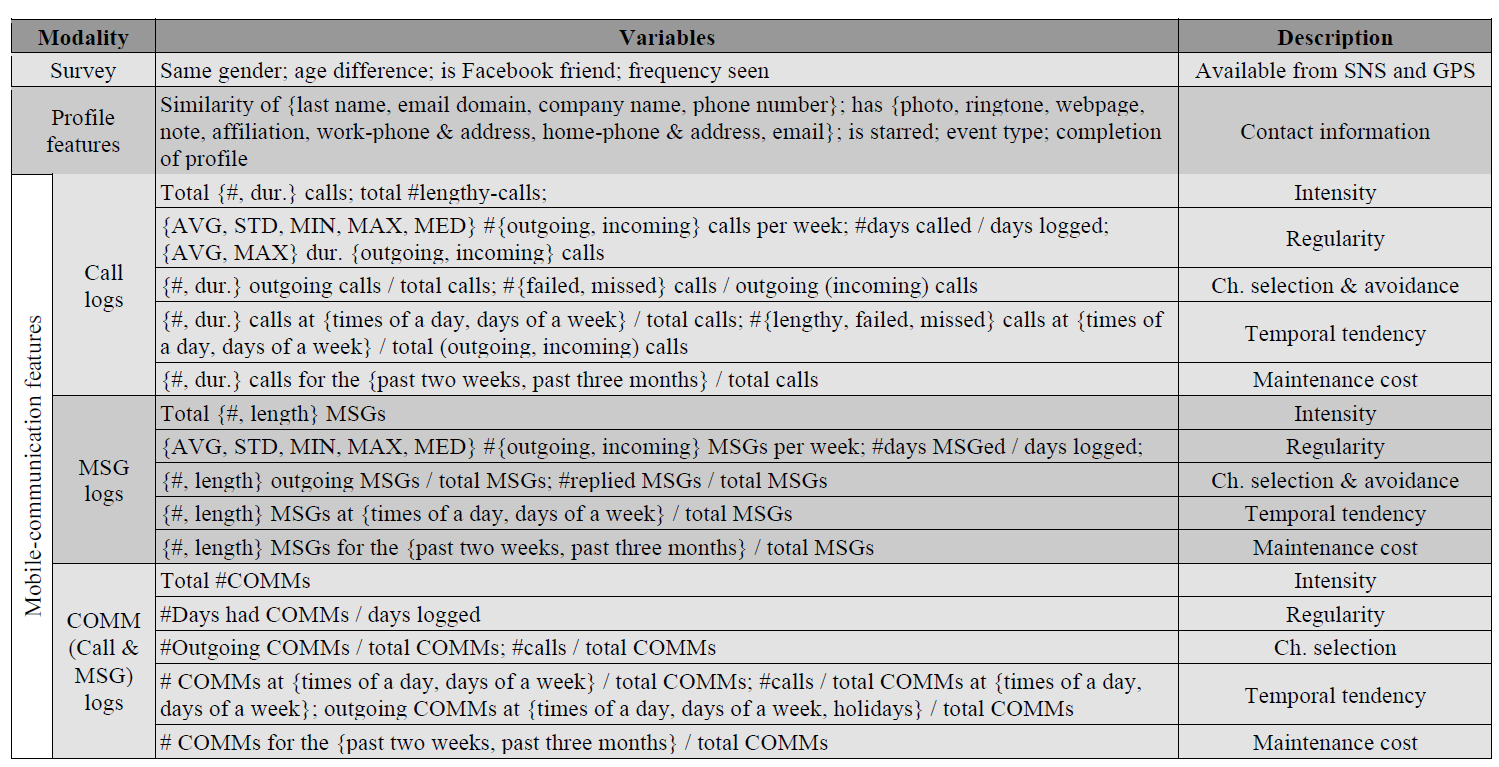
\includegraphics[width=1\textwidth]{figures/feature_extraction_placeholder.png}
    \caption{Table of extracted communication features, derived from~\cite{min2013mining}}.
    \label{fig:comm_features}
\end{figure*}

\pagebreak

\pagebreak

%\nocite{*} % for showing all references
\bibliographystyle{plain}
\bibliography{references}

\end{document}